% Mathe Formelsammlung für HM2 SoSe 2011
% 2 Seiten
% Copyrightrechte des Quellcodes besitzt www.latex4ei.de


% Dokumenteinstellungen
% ======================================================================

% Dokumentklasse (Schriftgröße 6, DIN A4, Artikel)
\documentclass[6pt,a4paper]{scrartcl}

% Zusätzliche Pakete laden
\usepackage[utf8]{inputenc}        % Zeichenkodierung: UTF-8 (für Umlaute)
\usepackage[german]{babel}        % Deutsche Sprache
\usepackage{multicol}            % Spaltenpaket
\usepackage{amsmath}            % erlaubt mathematische Formeln
\usepackage{amssymb}            % Verschiedene Symbole
\usepackage{esint}                % erweiterte Integralsymbole
\usepackage{booktabs}            % bessere Tabellenlinien
\usepackage{graphicx}            % Zum Bilder einfügen benötigt
\usepackage{color}                % Farbiger Text möglich
\usepackage{pbox}                % Intelligent parbox: \pbox{maximum width}{blabalbalb \\ blabal}
%\usepackage{undertilde}            % Für Welle unterhlab von Matrixbuchstaben benötigt
\usepackage{accents}            % Für eigene Ableitungspunkte benötigt
\usepackage{scrtime}
\usepackage{supertabular}        % Für lange Tabellen mit Umbruch
\usepackage{pdfpages}
\usepackage{trfsigns}            % Laplace und Fourier
\usepackage{array}


% Seitenlayout und Ränder:
\usepackage{geometry}
\geometry{a4paper,landscape, left=6mm,right=6mm, top=-1mm, bottom=3mm,includeheadfoot}
\setlength{\parindent}{0mm}


% Dokumentbeschreibung
\title{Formelsammlung Analysis 2 für EI}
\author{Emanuel Regnath}


% Kopf- und Fußzeile
% ======================================================================
\usepackage{fancyhdr}
\pagestyle{fancy}
\fancyhf{}
   \fancyfoot[C]{\textbf{Analysis 2} von Latex4ei (info@latex4ei.de)}
   \renewcommand{\headrulewidth}{0.0pt} %obere Linie ausblenden
   \renewcommand{\footrulewidth}{0.1pt} %obere Linie ausblenden

   \fancyfoot[R]{Stand: \todayV}
   \fancyfoot[L]{Homepage: www.latex4ei.de -  Fehler bitte \emph{sofort} melden.}
% ----------------------------------------------------------------------

% Ausgegraut zum Abschreiben:
%\definecolor{grey}{rgb}{0.6,0.6,0.6}
%\color{grey}

% Eigene Befehle und Befehlsüberschreibungen
% ======================================================================

% Schriftart SANS für bessere Lesbarkeit bei kleiner Schrift
\renewcommand{\familydefault}{\sfdefault}
% Array- und Tabellenabstände vergrößern
\renewcommand{\arraystretch}{1.2}

% Befehle sichern
\let\oldvec = \vec
\let\olddot = \dot

% Eigene Befehle
\newcommand{\todayV}{\the\day.\the\month.\the\year}                          %%D.M.YYYY

\newcommand{\iset}[2]{\ensuremath{\bigl\{ \bigl. #1 \, \bigr| \, #2 \bigr\}}}                   % intensional set
\newcommand{\eset}[1]{\ensuremath{\bigl\{#1\bigr\}}}                                            % extensional set
%\newcommand{\enbrace}[1]{\ensuremath{\bigl\(#1\bigr\)}}                                        % extensional set
\newcommand{\enbrace}[1]{\ensuremath{\left(#1\right)}}
\newcommand{\norm}[1]{\ensuremath{\|#1\|}}                                                      % Norm
\newcommand{\mat}[1]{\ensuremath{\begin{bmatrix} #1 \end{bmatrix}}}                             % Matrix
\newcommand{\ma}[1]{\ensuremath{\boldsymbol {#1}}}                                              % Matrixsymbol
\newcommand{\vect}[1]{\ensuremath{\begin{pmatrix} #1 \end{pmatrix}}}                            % Vektor
\newcommand{\mvect}[1]{\ensuremath{\left. \begin{matrix} #1 \end{matrix}  \right]}}             % Matrixvektornotation
\newcommand{\gk}[1]{\ensuremath{\left\lfloor#1\right\rfloor}}                                   % Gaußklammer
\newcommand{\sprod}[2]{\ensuremath{\left\langle #1, #2 \right\rangle }}                         % Skalarprodukt
\newcommand{\abs}[1]{\ensuremath{\left\vert#1\right\vert}}                                      % Betrag
\newcommand{\bdot}{\ensuremath{\boldsymbol \cdot}}                                              % Dicker Punkt für Skalarprodukt
\newcommand{\svdots}{\ensuremath{\olddot :}}                                                    % small vertical dots
\newcommand{\mustbe}{\stackrel{!}{=}}

\newcommand{\inn}{\operatorname{int}}


% Überschreibungen
\renewcommand{\vec}[1]{\ensuremath{\boldsymbol {#1}}}                                           % Vektor fett und unterstrichen
\renewcommand{\emph}[1]{\textbf{#1}}                                                            % Hervorhebungen fett
\renewcommand*{\dot}[1]{\accentset{\mbox{\textrm{\large\bfseries .}} }{#1}}                     % Dicker Ableitungspunkt
\renewcommand*{\ddot}[1]{\accentset{\mbox{\textrm{\large\bfseries .\hspace{-0.25ex}.}}}{#1}}    % Dicker Doppelableitungspunkt

% Abkürzungen
\newcommand{\ul}[1]{\ensuremath{\underline{#1}}}                               % Untersteichen
\newcommand{\ol}[1]{\ensuremath{\overline{#1}}}                                % Überstreichen
\newcommand{\Ra}[0]{\ensuremath{\Rightarrow}}                                  % Rightarrow
\newcommand{\ra}[0]{\ensuremath{\rightarrow}}                                  % Rightarrow
\newcommand{\bs}[1]{\ensuremath{\boldsymbol{#1}}}                              % Fett und kursiv im mathmode
\newcommand{\diff}{\ensuremath{\;\mathrm d}}                                   % differentielles delta
\newcommand{\grad}{\ensuremath{\mathrm{grad}\ }}                               % Gradient
\renewcommand{\div}{\ensuremath{\mathrm{div}\ }}                               % Divergenz
\newcommand{\rot}{\ensuremath{\mathrm{rot}\ }}                                 % Rotation
\newcommand{\Sp}{\ensuremath{\mathrm{Sp}\ }}                                   % Spur
\renewcommand{\i}{\ensuremath{\mathrm{i}}}                                     % Imaginäre Einheit

% Für Mengen
\newcommand{\N}{\ensuremath{\mathbb N}}
\newcommand{\R}{\ensuremath{\mathbb R}}
\newcommand{\C}{\ensuremath{\mathbb C}}


%Custom functions
\DeclareMathOperator{\arccot}{arccot}


% Dokumentbeginn
% ======================================================================
\begin{document}


% Aufteilung in Spalten
\begin{multicols*}{4}
    \parbox{2.3cm}{
        
\includegraphics[height=1.5cm]{./img/Logo.pdf}
    }
    \parbox{4cm}{
        \emph{\Large{Analysis 2}}
    }
    \vspace{-2mm} % Man muss optimieren wos nur geht ;)
    % -------------------------------------------
    % |         Mathematik 2                    |
    % ~~~~~~~~~~~~~~~~~~~~~~~~~~~~~~~~~~~~~~~~~~~
    %=======================================================================

    \section{Nützliches Wissen $e^{\i x} = \cos (x) + \i \cdot \sin(x)$}
    \if{0}
    \subsection{Trigonometrische Funktionen}
    \subsubsection{sinh, cosh \quad $\cosh^2(x)  \bs - \sinh^2(x) = 1$}
    $\sinh x = \frac{1}{2}(e^x -e^{-x}) \qquad \quad \operatorname{arsinh}\ x:= \ln\left(x+\sqrt{x^2+1}\right) \\
        \cosh x  = \frac{1}{2}(e^x +e^{-x}) \qquad \quad \operatorname{arcosh}\ x:= \ln\left(x+\sqrt{x^2-1}\right)\\
    $\\
    \begin{tabular}{ll}
        Additionstheoreme                         & Stammfunktionen                     \\
        $\cosh x \,\; + \sinh x \,\,= e^{x}$      & $\int \sinh x \, dx = \cosh x + C$  \\
        $\sinh({\rm arcosh}(x)) = \sqrt{x^2 - 1}$ & $\int \cosh x \, dx = \sinh x + C $ \\
        $\cosh({\rm arsinh}(x)) = \sqrt{x^2 + 1}$                                       \\
    \end{tabular}
    %Kugel: $V_K = \frac{4}{3} \pi r^3$ \qquad $A_K = 4 \pi r^2$
    %\subsection{subsection name} % (fold)
    %\label{sub:subsection name|\(.)|(\w+)|([^\w\]+)/(?4:_:\L$1$2$3)/g}}

    % subsection |\(.)|(\w+)|([^\w\]+)/(?4:_:\L$1$2$3)/g (end)

    \subsubsection{sin, cos \quad $\sin^2(x) \bs + \cos^2(x) = 1$}
    $\begin{array}{c|c|c|c|c|c|c|c|c}
            x    & 0 & \pi / 6            & \pi / 4            & \pi / 3           & \pi / 2 & \pi & \frac{3}{2}\pi & 2 \pi \\ \hline
            \sin & 0 & \frac{1}{2}        & \frac{1}{\sqrt{2}} & \frac{\sqrt 3}{2} & 1       & 0   & -1             & 0     \\
            \cos & 1 & \frac{\sqrt 3}{2}  & \frac{1}{\sqrt 2}  & \frac{1}{2}       & 0       & -1  & 0              & 1     \\
            \tan & 0 & \frac{\sqrt{3}}{3} & 1                  & \sqrt{3}          & \infty  & 0   & - \infty       & 0     \\
        \end{array}$
    \begin{tabular}{l  l}
        Additionstheoreme                   & Stammfunktionen                                                    \\
        $\cos (x - \frac{\pi}{2}) = \sin x$ & $\int x \cos(x) \diff x = \cos(x) + x \sin(x)$                     \\

        $\sin (x + \frac{\pi}{2}) = \cos x$ & $\int x \sin(x) \diff x = \sin(x) - x \cos(x)$                     \\

        $\sin 2x = 2 \sin x \cos x $        & $\int \sin^2(x) \diff x = \frac12 \bigl(x - \sin(x)\cos(x) \bigr)$ \\

        $\cos 2x = 2\cos^2 x - 1$           & $\int \cos^2(x) \diff x = \frac12 \bigl(x + \sin(x)\cos(x) \bigr)$ \\

        $\sin(x) = \tan(x)\cos(x)$          & $\int \cos(x)\sin(x) = -\frac12 \cos^2(x)$                         \\
    \end{tabular}

    \subsection{log \quad $\log(1) = 0$}
    $a^x = e^{x \ln a} \qquad \quad \log_a x = \frac{\ln x}{\ln a} \qquad \quad \ln x \le x -1$

    \subsection{Quadratische Gleichung}
    $x_1,_2 = \frac{-b \pm \sqrt{b^2 - 4ac}}{2a}$

    \subsection{Ableitungsregeln:}
    Linearität: $(\lambda f + \mu g)' (x) = \lambda f'(x) + \mu g'(x)$ \quad $\forall \lambda, \mu \in \mathbb R$ \\
    Produktregel: $(f \cdot g)' = f' g + f g'$\\
    Quotientenregel $\enbrace{\frac{f}{g}}' = \frac{f'g - fg'}{g^2}$\\
    Kettenregel: $\left( f(g(x)) \right)' = f'(g(x)) g'(x)$\\
    Potenzreihe: $f: ] \underbrace{-R+a, a+R}_{\subseteq D}     [ \rightarrow \mathbb R, f(x) = \sum_{n=0}^{\infty} a_n (x -a)^n$ \quad $\Rightarrow$ \quad $f'(x) = \sum_{n=0}^{\infty} n a_{n} (x-a)^{n-1}$\\
    \textbf{Tangentengleichung:} $y=f(x_0)+f'(x_0)(x-x_0)$
    \fi

    \subsection{Integrale:}
    \begin{itemize}\itemsep-1pt
        \item Partielle Integration: $\int uv'=uv-\int u'v$
        \item Substitution: $\int f(\underbrace {g(x)}_{t}) \underbrace {g'(x)\,\mathrm dx}_{\mathrm dt}=\int f(t)\, \mathrm dt$
    \end{itemize}

    $\int_a^b f(x) \mathrm dx = F(b) - F(a)$\\
    $\int\lambda f(x)+\mu g(x) \, \mathrm dx=\lambda\int f(x) \, \mathrm dx + \mu\int g(x) \, \mathrm dx$

    \everymath{\displaystyle}    % Formeln ab hier groß Schreiben
    \begin{math}\renewcommand{\arraystretch}{1.8}
        \begin{array}{c|c|c}
            F(x)                                               & f(x)        & f'(x)                                    \\ \hline
            \frac{1}{q+1}x^{q+1}                               & x^q         & qx^{q-1}                                 \\
            \raisebox{-0.2em}{$\frac{2\sqrt{ax^3}}{3}$}        & \sqrt{ax}   & \raisebox{0.2em}{$\frac{a}{2\sqrt{ax}}$} \\
            x\ln(ax) -x                                        & \ln(ax)     & \textstyle \frac{a}{x}                   \\
            e^x                                                & e^x         & e^x                                      \\
            \frac{a^x}{\ln(a)}                                 & a^x         & a^x \ln(a)                               \\
            -\cos(x)                                           & \sin(x)     & \cos(x)                                  \\
            \sin(x)                                            & \cos(x)     & -\sin(x)                                 \\
            -\ln |\cos(x)|                                     & \tan(x)     & \frac{1}{\cos^2(x)}                      \\
            \ln |\sin(x)|                                      & \cot(x)     & \frac{-1}{\sin^2(x)}                     \\
            x\arcsin (x)+\sqrt{1-x^2}                          & \arcsin(x)  & \frac{1}{\sqrt{1-x^2}}                   \\
            x\arccos (x)-\sqrt{1-x^2}                          & \arccos(x)  & -\frac{1}{\sqrt{1-x^2}}                  \\
            x\arctan (x)-\frac{1}{2} \ln \left| 1+ x^2 \right| & \arctan (x) & \frac{1}{1+x^2}                          \\
            x\arctan (x)+\frac{1}{2} \ln \left| 1+ x^2 \right| & \arccot (x) & -\frac{1}{1+x^2}                         \\
            \sinh(x)                                           & \cosh(x)    & \sinh (x)                                \\
            \cosh(x)                                           & \sinh(x)    & \cosh (x)                                \\
        \end{array}
    \end{math}
    \everymath{\textstyle}

    \if{0}
    \subsection{Reihen}

    $\underset{\text{Harmonische Reihe}}{\sum\limits_{n=1}^\infty \frac{1}{n} \ra \infty} \qquad   \underset{\text{Geometrische Reihe}}{\sum\limits_{n=0}^\infty q^n \stackrel{|q|<1}= \frac{1}{1-q}}  \qquad \underset{\text{Exponentialreihe}}{\sum\limits_{n = 0}^{\infty} \frac{z^n}{n!} = e^z}$

    \section{Kurven}
    %===========================================================================================================================================================
    Eine Kurve ist ein eindimensionales Objekt.\\
    $ \vec \gamma:[a,b] \rightarrow \mathbb R^n, t \mapsto \begin{pmatrix} \gamma_1(t) \\ \svdots \\ \gamma_n(t) \end{pmatrix} \quad \text{(Funktionenvektor)} $
    %Eigenschaften von Kurven:
    \begin{itemize}\itemsep-2pt
        \item $\mathcal C^0$-Kurve: Positionsstetigkeit (geschlossene Kurve)
        \item $\mathcal C^1$-Kurve: Tangentialstetigkeit (stetig diffbar)
        \item $\mathcal C^2$-Kurve: Krümmungsstetigkeit (2 mal stetig diffbar)
        \item regulär, falls $\forall t \in [a,b]:\dot \gamma(t) \ne \vec 0$ (Keine Knicke)
    \end{itemize}
    Besondere Punkte von Kurven:
    \begin{itemize}\itemsep-2pt
        \item Singulär, falls $\dot \gamma(t)=\vec 0$ (Knick)
        \item Doppel-punk, falls $\exists t_1,t_2:t_1 \ne t_2 \ \land \ \gamma(t_1)=\gamma(t_2)$
        \item Horizontaler Tangentenpunkt, falls $\dot \gamma_1(t) \ne 0 \ \land \ \dot \gamma_2(t)=0$
        \item Vertikaler Tangentenpunkt, falls $\dot \gamma_1(t) = 0 \ \land \ \dot \gamma_2(t) \ne 0$
    \end{itemize}
    \emph{Bogenlänge} einer Kurve: $L(\gamma) = \int_{a}^{b} \norm{\dot \gamma(t)} \mathrm dt$ \\


    Umparametrisierung $\gamma$ nach Bogenlänge ($\tilde \gamma$):
    \begin{itemize} \itemsep0pt
        \item Bogenlängenfunktion: $s(t) = \int\limits_a^t \norm{\dot \gamma(\tau)} \mathrm d\tau$\\
              $s: [a,b] \ra [0,L(\gamma)], t \mapsto s(t)$
              %\item Umkehrfunktion: $s^{-1}:[0,L(\gamma)] \rightarrow [a,b]$ (streng monoton wachsend)
        \item $\tilde \gamma(t)=\gamma \bigl(s^{-1}(t) \bigr)$ \qquad $\norm{\ \dot{\tilde \!\! \gamma \!}\; (t)}=1 \forall t$ % Hässlich wie die Nacht aber geht iwie nicht anders...
    \end{itemize}
    Tangenteneineitsvektor an $\gamma(t): T(t)=\frac{\dot \gamma(t)}{\norm{\dot \gamma(t)} }$\\
    Krümmung von $\gamma$: $\kappa(t)= \norm{\frac{\mathrm d^2 \gamma}{\mathrm d s^2}} = \frac{\norm{\dot T(t)}}{s'(t)}$\\
    \\
    \textbf{Vereinfachung} für $n=2$: $\gamma:[a,b] \rightarrow \mathbb R^2, t \mapsto \bigl(x(t),y(t)\bigr)$ \\
    \everymath{\displaystyle}    % Formeln ab hier groß Schreiben
    \boxed{ L(\gamma) = \int_a^b \sqrt{\dot x^2 + \dot y^2}\; \mathrm dt$ \qquad $\tilde{\kappa}(t)=\frac{\dot x \ddot y - \ddot x \dot y}{(\dot x^2 + \dot y^2)^{\frac{3}{2}}} } \\
    \everymath{\textstyle}
    % \subsection{Funktionen als Kurve}
    % Funktion $f$ als Kurve: $\gamma:[a,b] \rightarrow \mathbb R^2, t \mapsto \begin{pmatrix} t \\ f(t) \end{pmatrix}$\\
    % Länge von $f$: $L(\gamma) = \int_a^b \sqrt{1+f'(t)^2}\; \mathrm dt$ \qquad Krümmung von $f$: $\varkappa(t)=\frac{f''(t)}{\sqrt{(1+f'(t)^2)^3}}$\\

    \fi

    \section{Skalarfelder}
    %===========================================================================================================================================================
    Ein Skalarfeld ordnet jedem Vektor eines Vektorraums einen Wert zu.\\
    $ f:D\subseteq \mathbb R^n \rightarrow \mathbb R, (x_1,\ldots ,x_n)^T \mapsto f(x_1,\ldots ,x_n) $
    \parbox{5.5cm}{
    Teilmengen von $\mathbb R^n$: $D = [a_1,b_1] \times ... \times [a_n,b_n]$\\
    Offene Kugelmenge vom Radius $r$: $B_r(x_0)$\\
    \emph{Topologische Begriffe} für $D \subseteq \mathbb R^n$ } \parbox{1.0cm}{ 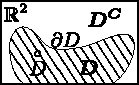
\includegraphics[height=0.8cm]{img/topologie.pdf} }
    \begin{itemize}\itemsep-1pt
        \item Das Komplement $D^C$ von $D$: $D^C := \R^n \setminus D$
        \item innerer Punkt $x_0 \in \mathbb R^n$ des Inneren $\inn(D)$, falls \\
              $\exists \varepsilon > 0: B_\varepsilon (x_0) = \iset{x\in \mathbb R^n}{\norm{x-x_0} < \varepsilon} \subseteq D$
        \item Die Menge $D$ heißt offen, falls $D=\inn(D)$
        \item Randpunkt $x_0 \in \mathbb R^n$ des Rands $\partial D$ von $D$, falls $\forall \varepsilon > 0:$ \\
              $B_\varepsilon(x_0) \cap D \ne \emptyset \ \land \ B_\varepsilon(x_0) \cap D^C \ne \emptyset \ \Rightarrow \ \partial D = \partial D^C$
        \item Abschluss $\ol D$ von $D$: $\overline{D}=D \cup \partial D$
        \item Die Menge $D$ ist abgeschlossen, falls $\partial D \subseteq D$
        \item beschränkt, falls $\exists \mu \in \mathbb R \quad \forall x \in D: \norm{x} < \mu$
        \item kompakt, falls D abgeschlossen und beschränkt ist.
    \end{itemize}
    Es gilt: Ist $D \subseteq \mathbb R^n$ offen, so ist $D^C$ abgeschlossen. \\
    $\mathbb R$ und $\emptyset$ sind offen und abgeschlossen.

    \subsection{Folgen, Grenzwerte, Stetigkeit im $\mathbb R^n$}
    %-----------------------------------------------------------------------
    Eine Folge $(a_n)$ ist eine Abbildung $(a_n):\mathbb N_0 \rightarrow \mathbb R^n, k\mapsto a_n$\\
    %Die Folge konvergiert, falls $\lim\limits_{k \rightarrow \infty} \norm{x-x^{(k)}} = 0$\\
    %Folge konvergiert, falls sie komponentenweise konvergiert!\\
    %\\
    Für $f:D \subseteq \mathbb R^n \rightarrow \mathbb R$ bedeutet \\
    Grenzwert: \quad  $\lim\limits_{x \rightarrow x_0} f(x) =c \Leftrightarrow f a_n \rightarrow x_0 \bigr) \rightarrow c\quad \forall a_n$\\
    Stetigkeit: \quad \ $\forall x \in \mathbb R^n:\lim\limits_{x \rightarrow x_0} f(x) = f(x_0)$\\
    Satz von Max. und Min.: Ist $f(\vec x)$ stetig und $D$ kompakt, so\\
    % Ist $f:D \subseteq \mathbb R^n \rightarrow \mathbb R$ stetig und D kompakt, so\\
    $\exists x_{max},x_{min} \in D \quad \forall x\in D:f(x_{\text{min}}) \le f(x) \le f(x_{\text{max}})$

    \subsection{Differentiation von Skalarfeldern - Gradient}
    %-----------------------------------------------------------------------
    % \boxed {f_{x_i}(x)=\lim\limits_{h \rightarrow 0} \frac{f(x+he_i)-f(x)}{h}}\\
    $\nabla f(x) = \mathrm{grad} \bigl( f(x) \bigr) = \begin{pmatrix}  \frac{\partial}{\partial x_1} f(x) \\ \svdots \\ \frac{\partial}{\partial x_n} f(x) \end{pmatrix}$\\
    \emph{Richtungsableitung:} \boxed { \partial_{\vec v} f(x) = \left\langle \nabla f(x), \vec v \right\rangle } \quad \boxed{ \norm{\vec v}=1 }\\
    \\
    \\
    \textbf{Gradientenregeln:} $f,g:D \subseteq \mathbb R^n \rightarrow \mathbb R$ sind partiell diffbar:\\
    Linearität: $\nabla(\lambda f + \mu g) (x) = \lambda \nabla f(x) + \mu \nabla g(x)$\\
    Produkt: $\nabla (f \cdot g) (x) = g(x) \nabla f(x) + f(x) \nabla g(x)$\\
    Quotient: $\nabla \Bigl( \frac{f}{g} \Bigr) = \frac{1}{g^2} \bigl( g(x)\nabla f(x) - f(x) \nabla g(x) \bigr)$\\
    \\
    Kettenregel\textbf{n:}\\
    \begin{tabular}{l|l}
        $f:\mathbb R^n \rightarrow \mathbb R \land g:\mathbb R \rightarrow \mathbb R$ & $f:\mathbb R^n \rightarrow \mathbb R \land g:\mathbb R \rightarrow \mathbb R^n$ \\ \midrule
        $h:= g \circ f: \mathbb R^n \rightarrow \mathbb R$                            & $h:= f \circ g: \mathbb R \rightarrow \mathbb R$                                \\
        $\boxed{ \nabla h(x) = g'\big( f(x) \big) \cdot \nabla f(x)}$                 & $\boxed{h'(x)=\nabla f\big( g(x) \big)^T \cdot g'(x)}$
    \end{tabular}


    \subsection{Differentialoperatoren \qquad $\div(\rot(f)) = 0$}
    \begin{tabular}{l|l}
        Operator & Definition                       \\ \midrule
        \pbox{2.0cm}{ Gradient: $\mathrm{grad}\; f$ \\ S-Feld $\rightarrow$ V-Feld } & $\nabla f = \vect{\partial_1 f \\ \svdots \\ \partial_n f}$ \\ \midrule
        \pbox{2.0cm}{ Divergenz: $\mathrm{div}\; f$ \\ V-Feld $\rightarrow$ S-Feld } & ${\displaystyle \nabla^\top \bdot f = \sum\limits_{i=0}^n \partial_i f_i}$\\ \midrule % \vect{\frac{\partial}{\partial x_1} \\ \svdots \\ \frac{\partial}{\partial x_n} }^\top \bdot \vect{ f_1 \\ \svdots \\ f_n }$ \\ \midrule
        \pbox{2.0cm}{ Rotation: $\mathrm{rot}\; f$  \\ V-Feld $\rightarrow$ V-Feld } & $\nabla \times f = \vect{\partial_2 f_3(x) - \partial_3 f_2(x) \\[2pt] \partial_3 f_1(x) -\partial_1 f_3(x) \\[2pt] \partial_1 f_2(x) -\partial_2 f_1(x) }$ \\ \midrule
        \pbox{2.0cm}{ Laplace: $\Delta\; f$         \\ S-Feld $\rightarrow$ S-Feld } & ${\displaystyle\underset{\nabla^\top \cdot (\nabla f)}{\nabla^2} = \sum \partial_i^2 f}$ % \vect{\frac{\partial}{\partial x_1} \\ \svdots \\ \frac{\partial}{\partial x_n} }^\top \cdot \vect{\frac{\partial f}{\partial x_1} \\ \svdots \\ \frac{\partial f}{\partial x_n} }$ \\
    \end{tabular}


    \subsection{Höhere Partielle Ableitungen $\partial_j \partial_i f(x) = f_{x_i x_j} (x)$}
    %-----------------------------------------------------------------------
    $\mathcal C^m (D) = \eset{\text{m-mal stetig partiell diffbare Funktion auf D}}$\\
    Satz von Schwarz: $f \in \mathcal C^2 (D) \Rightarrow f_{x_i x_j} (x)= f_{x_j x_i} (x) \quad \forall i,j$\\
    \\
    Mittelwertsatz ($f:D\subseteq \mathbb R^n \rightarrow \mathbb R, xy \in D \quad x,y \subseteq D$)\\
    $\exists \xi \in \overline{x,y}$ mit $f(y)-f(x)=\nabla f^\top (\xi)(y-x)$\\
    Es gilt $|f(y) - f(x)| \le c|y-x|$ mit $c= \mathrm{max} \norm{\nabla f(z)} \quad z \in \overline{x,y}$\\
    \\
    Hessematrix: $H_f (x) = \nabla^2 f(x) = \begin{bmatrix} \partial_{11} f(x)\ ...\ \partial_{1n} f(x) \\ \svdots \quad \qquad \qquad \svdots \\ \partial_{n1} f(x)\ ...\ \partial_{nn} f(x) \end{bmatrix}$\\
    Die Hessematrix ist symmetrisch, falls $f \in \mathcal C^2(D)$\\
    \\
    \begin{tabular}{ll}
        $T_{2,f, \vec x_0} (\vec x) =$ $f(\vec x_0) +$                                                  \\
        \qquad $+ \nabla f(\vec x_0)^\top (\vec x-\vec x_0) +$                      & (Tangentialebene) \\
        \qquad $+ \frac{1}{2}(\vec x-\vec x_0)^\top \ma H_f(x_0)(\vec x- \vec x_0)$ & (Schmiegequadrik) \\
        %\qquad $+ \qquad \svdots$ & (räumliche Matrix)\\
    \end{tabular}

    $T_{3,f,\vec a}(\vec x) = f(\vec a) + \sum \partial_i f(\vec a)(x_i - a_i) + \frac{1}{2} \sum \partial_i \partial_j f(\vec a)(x_i - a_i)(x_j - a_j) + \frac{1}{6} \sum \partial_i \partial_j \partial_k f(\vec a)(x_i - a_i)(x_j - a_j)(x_k - a_k)$

    \subsection{Jacobimatrix = Fundamentalmatrix}
    $\ma J_f (x) = \begin{bmatrix} \frac{\partial f_1}{\partial x_1} & ... & \frac{\partial f_1}{\partial x_n} \\ \svdots & & \svdots \\ \frac{\partial f_m}{\partial x_1} & ... & \frac{\partial f_m}{\partial x_n} \end{bmatrix} = \begin{pmatrix} \nabla f_1^\top \\ \svdots \\ \nabla f_m^\top \end{pmatrix}  \quad \in \mathbb R^{m \times n}$\\ \\
    Rechenregeln für die Jacobimatrix:\\
    $f,g: D \subseteq \mathbb R^n \rightarrow \mathbb R^m$ part. diffbar:\\
    Linearität: $\ma J_{\alpha f + \beta g} = \alpha J_f + \beta J_g$\\
    Produkt: $\ma J_{f^\top g} = g^\top J_f + f^\top J_g$ \quad $(\nabla f^\top g = J_f^\top g + J_g^\top f)$\\
    Komposition: $\ma J_{g \circ f}(x) = \ma J_g\Bigl(f(x)\Bigr) \cdot \ma J_f(x)$\\
    Umkehrfunktion: $\ma J_{f^{-1}} (f(x)) = \ma J_f (x)^{-1}$

    \if{0}
    \subsection{Lineare Abbildungen}
    %-----------------------------------------------------------------------
    $f:V \rightarrow W$ heißt linear, falls

    \begin{itemize}\itemsep0pt
        \item $f(v+w) = f(v) + f(w)$
        \item $f(\lambda v) = \lambda f(v)$
        \item Tipp: Prüfe ob $f(0) = 0$
    \end{itemize}
    Kern von $f$: $\ker (f) = \iset{v \in V}{f(v) = 0}$ ist UVR von $V$\\
    Bild von $f$: $\mathrm{Bild}(f) = \iset{f(v)}{v \in V}$ ist UVR von $W$\\
    \emph{Dualraum} $V^* = \iset{f:\mathbb R^n \rightarrow \mathbb R}{f=lin.}$\\
    \emph{Injektiv} (aus $f(x) = f(y) \ra x = y)$), falls $\ker(f) = \eset{0}$ \\
    \emph{Surjektiv} Alle Werte im Zielraum werden angenommen.
    \fi

    \section{Taylorpolynom für Skalarfelder}
    %===========================================================================================================================================================
    Ist $f:D\subset \mathbb R^n \rightarrow \mathbb R$ ein ($m+1$)-mal stetig partiell differenzierbar Skalarfeld, D offen und konvex, so gilt für alle $\vec a \in D$ und $\vec h \in \mathbb R^n$ mit $\vec a + \vec h \in D$ die Approximation durch das Taylorpolynom :
    \boxed{ \ T_m(\vec a; \vec a + \vec h) = g(0) + g'(0) + \frac{1}{2} g''(0) + \dots + \frac{1}{m!}g^{m}(0)} \\
    (Teilen durch $n!$ nicht vergessen!) \\ \\
    $g:[0,1] \rightarrow \mathbb R$ ist definiert als $g(t) = f(a+th)$ \\
    Die Ableitungen von $g$ an der Stelle $0$ können wie folgt bestimmt werden:

    \begin{itemize}
        \item $g(0) = f(\vec a)$
        \item $g'(0) = \nabla f(\vec a)^\top \vec h = \sum_{i=1}^{n}\partial _{x_i} f(\vec a)h_i$
        \item $g''(0) = h^\top H_f(\vec a) \vec h = \sum_{i,j=1}^{n} \partial_{x_j}\partial_{x_i}f(\vec a)h_i h_j$
        \item $g'''(0) = \sum_{i,j,k=1}^{n} \partial_{x_i}\partial_{x_j}\partial_{x_k}f(\vec a)h_i h_j h_k$
        \item \dots
    \end{itemize}

    \subsection{Das Restglied - die Taylorformel}
    \begin{equation*}
        \begin{split}
            R_{m+1}(a; a+h) &= f(x)- T_m(a,a+h) \\
            &= \frac{1}{m!} \int_{0}^{1}(1-t)^m g^{(m+1)}(t)\mathrm dt
        \end{split}
    \end{equation*}

    Es gibt eine Zwischenstelle $\xi \in (0,1)$ mit: \\
    \begin{equation*}
        R_{m+1}(a; a+h) = \frac{1}{m!} g^{(m+1)}(\xi)
    \end{equation*}



    % evtl. nochmal anschauen
    \section{Koordinatensysteme}
    %===========================================================================================================================================================
    Transformationsvektoren (Um einen Vektor in anderen Koordinaten darzustellen):\\ \\
    \begin{tabular}{c | c  l}
                 & $(x, y, z)^\top$             &                              \\ \midrule
        Zylinder & $\begin{pmatrix} r \cdot \cos (\varphi) \\ r \cdot \sin (\varphi) \\ z \end{pmatrix}$ & $0 \le \varphi < 2 \pi$      \\
        Kugel    & $\begin{pmatrix} r \cdot \cos(\varphi) \sin(\theta) \\ r \cdot \sin(\varphi) \sin(\theta) \\ r \cdot \cos(\theta) \end{pmatrix}$ & $\begin{matrix}0 \le \varphi < 2 \pi \\ 0 \le \theta \le \pi \end{matrix}$
    \end{tabular} \\ \\
    \\

    Transformationsmatrix $\ma S_z$ \\
    $\mat{ \vec e_r & \vec e_\varphi & \vec e_z} = \mat{ \cos(\varphi) &  -\sin(\varphi) & 0\\ \sin(\varphi) & \cos(\varphi) & 0 \\ 0 & 0 & 1 }$
    \begin{center}
        \boxed{f_{\text{kart}} = \ma S_z \cdot f_{\text{zyl}} \qquad \qquad f_{\text{zyl}} = \ma S_z^{-1} \cdot f_{\text{kart}}} \\
    \end{center}
    \qquad \\ \\
    Transformationsmatrix $\ma S_k$ \\
    $\mat{ \vec e_r & \vec e_\theta & \vec e_\varphi} =
        \mat{ \cos(\varphi) \sin(\theta) & \cos(\varphi)\cos(\theta)  & - \sin(\varphi)\\
            \sin(\varphi)\sin(\theta) & \sin(\varphi)\cos(\theta)  & \cos(\varphi)\\
            \cos(\theta) & - \sin(\theta)  & 0}$
    \\
    \begin{center}
        \boxed{f_{\text{kart}} = \ma S_k \cdot f_{\text{kug}} \qquad \qquad f_{\text{kug}} = \ma S_k^{-1} \cdot f_{\text{kart}}} \\
    \end{center}
    Die Spalten entsprechen den orthonormalen Basisvektoren im jeweiligen Koordinatensystem. \\ $\Ra$ Trafo-Matrizen orthogonal: $\ma S^{-1} = \ma S^\top$
    \if{0}
    \subsection{Transformation eines Skalarfeldes $f(x,y,z)$}
    $\tilde{f}(r,\varphi,z)$ bzw.  $\tilde{f}(r,\theta,\varphi)$ erhält man durch ersetzen von $x$, $y$ und $z$ durch die entsprechenden Einträge des Transformationsvektors.


    \subsection{Transformation eines Vektorfeldes $\vec f(x,y,z)$ }
    $\tilde{\vec f}(r,\varphi,z)$ bzw. $\tilde{\vec f}(r,\theta,\varphi)$ durch ersetzen von $x$, $y$ und $z$ durch die entsprechenden Einträge des Transformationsvektors. \\ \\
    Zylinder: $ \hat{\vec f}(r,\varphi,z)$ bzgl. $\{e_r,e_\varphi,e_z\}$: $\hat{\vec f} = \ma S_z^{-1} \cdot \tilde{\vec f}$ \\ \\
    Kugel: $\hat{\vec f}(r,\theta,\varphi)$ bzgl. $\{e_r,e_\theta,e_\varphi\}$: $\hat{\vec f} = \ma S_k^{-1} \cdot \tilde{\vec f}$

    \subsection{Operatoren in anderen Koordinaten}
    (Detailliert in der Formelsammlung im Anhang) \\ \\
    \begin{tabular}{c|l}
                  & Zylinderkoordinaten                                                                                             \\ \midrule
        $\nabla$  & $(\partial_r,\ \frac{1}{r}\partial_\varphi,\ \partial_z)^\top$                                                  \\ \midrule
        $\div$    & $\frac{1}{r} \partial_r(r\cdot \vec f_r) + \frac{1}{r} \partial_\varphi(\vec f_\varphi) + \partial_z(\vec f_z)$ \\ \midrule
        $ \Delta$ & $\frac{1}{r} \partial^2_{r}(r\cdot f) + \frac{1}{r^2} \partial^2_{\varphi}f + \partial^2_{z}f$
    \end{tabular}
    \\ \\ \\
    \begin{tabular}{c|l}
                  & Kugelkoordinaten                                                                                                                                                              \\ \midrule

        $\nabla$  & $(\partial_r,\ \frac{1}{r}\partial_\varphi,\ \frac{1}{r\sin\theta}\partial_\theta)^\top$                                                                                      \\ \midrule
        $\div$    & $  \frac{1}{r^{2}}  \partial_r(r^2 \vec f_r) + \frac{1}{r \sin \theta} \partial_\varphi(\vec f_\varphi) + \frac{1}{r \sin \theta} \partial_\theta(\sin \theta \vec f_\theta)$ \\ \midrule
        $\Delta $ & $ \frac{1}{r^{2}} \partial^2_{r}(r^2 f) + \frac{1}{r^2\sin^2\theta} \partial^2_{\varphi} (\sin\theta f) + \frac{1}{r^2\sin\theta} \partial^2_{\theta} f$
    \end{tabular}
    \fi

    \section{Implizite Funktionen $g$}
    %===========================================================================================================================================================
    ... werden als Nullstellenmenge einer expl. Funktion $f$ angegeben.\\
    $\iset{(x,y) \in \mathbb R^2 }{f(x,y) = 0}$ mit $y=g(x) \in \mathbb R$

    \subsection{Satz über implizite Funktionen}
    Es gelte: $f: D \in \mathbb R^2 \ra \mathbb R$ \quad
    $\ra $ implizite Gleichung $f(x,y) = 0$ \\
    Bedinungen für die Existenz von $y = g(x)$:
    \begin{itemize} \itemsep0pt
        \item $D$ ist offen
        \item $f \in C^1 (D)$
        \item $\exists (x_0, y_0) \in D$ mit $f(x_0, y_0) = 0$
        \item $f_y(x_0, y_0) \not = 0$
    \end{itemize}
    \emph{$\Ra$} $ \exists I \subseteq \mathbb D: I = (x_0 - \epsilon, x_0 + \epsilon) , J \subseteq \mathbb R: J = (y_0 - \delta, y_0 + \delta)$ mit:
    \begin{itemize}\itemsep0pt
        \item $I \times J \subseteq D$ in $f_y (x,y) \not = 0 \forall (x,y) \in I \times y$
        \item $\exists_1$ Funktion $g(x)$ mit $f(x,g(x)) = 0$ ("$g$ wird implizit defniert")
        \item $g'(x) = \frac{-f_x(x, g(x))}{f_y (x, g(x))} = \frac{-f_x(x, y)}{f_y (x, y)} \quad \forall x \in I$
    \end{itemize}


    $g''(x) = - \frac{f_{xx} (x, g(x)) + 2f_{xy}(x,g(x)) \cdot g'(x) + f_{yy} (x, g(x)) \cdot (g'(x))^2}{f_y (x, g(x))} $

    \subsection{Satz über implizite Funktionen (allgemein)}
    $f: \mathbb R^{k+m} \ra \mathbb R^m$ stetig diffbar,\\ $z_0 = (x_0, y_0) \in \mathbb R^{k+m}$      $x_0 \in \mathbb R^k, y_0 \in \mathbb R^m$ mit $f(z_0) = 0$
    \\
    Falls $J_{f,y} = (\frac{\partial f_{i(z_0)}}{\partial x_j})_{i = 1 \ldots m j= k +1 \ldots k+m}$ ist invertierbar $(\det J_{f,y} (z_0) \not = 0)$
    \\
    Dann: $\quad \exists$ offende Menge $I$ in $J$ mit $g: I \ra J$ mit $f(x,g(x)) = 0$


    \subsection{Satz von der Umkehrabbildung}

    $D \subseteq \mathbb R^n$ offen, $f: D \ra \mathbb R^n \in C^1 (D). X_0 \in D$ mit $J_f (x_0)$ ist invertierbar. \\
    Dann: $\exists U$ Umgebung von $x_0$ mit $f |_U : U \ra f(U)$ ist bijektiv. \\
    Die Umkehrfunktion $(f|_u)^{-1}$ ist stetig diffbar und es gilt: \\
    $J(f|_U)^{-1} (f(x)) = (J_f (x))^{-1} \forall x \in U$

    \section{Matrizen}

    \if{0}
    \subsection{Determinante von $A\in \mathbb K^{n\times n}$: $\det(A)=|A|$}

    $\det\begin{pmatrix}A&0\\C&D\end{pmatrix}=\det\begin{pmatrix}A&B\\0&D\end{pmatrix}=\det(A)\cdot\det(D)$ \\
    Hat $\ma A$ 2 linear abhäng. Zeilen/Spalten $\Rightarrow |A|=0$ \\
    Entwicklung. n. $i$ter Zeile: $|A|=\sum\limits_{i=1}^n (-1)^{i+j} \cdot a_{ij} \cdot |A_{ij}|$ \qquad


    \subsection{Eigenwerte, Eigenvektoren}
    \emph{Eigenwerte:} $\det(\ma A - \lambda \ma 1) = 0$, Det-Entwickl., Polynom-Div. \\
    $\Ra$ $\chi_A = (\lambda_1 - \chi)^{\nu_1} \cdot ... \cdot (\lambda_r - \chi)^{\nu_r}$ \quad $\nu_i = \mathrm{alg}(\lambda_i)$\\ \\
    \emph{Eigenvektoren:} $\mathrm{Eig}_A (\lambda_i) = \ker(\ma A - \lambda_i \ma 1) = v_i$\\
    $\ra \dim(\mathrm{Eig}_A (\lambda_i)) = \mathrm{geo}(\lambda_i)$ \quad $\forall i : 1 \le \mathrm{geo}(\lambda_i) \le \mathrm{alg}(\lambda_i)$\\ \\
    \boxed{\ma A \vec v = \lambda \vec v} mit $\vec v$ EV von $\ma A$ \\
    \underline{Ähnlichkeit von Matrizen:} Matrizen A und B sind ähnlich, wenn
    \begin{itemize}
        \item sie die gleichen Eigenwerte besitzen
        \item die algebraischen mit den geometrischen Vielfachheiten der Eigenwerte übereinstimmen
        \item Es gilt: $\det A = \det B$
    \end{itemize}

    \subsection{Diagonalmatrix}

    \underline{Bedingungen für Diagonalisierbarkeit:}
    \begin{itemize} \itemsep0pt
        \item Das charakteristische Polynom $\chi_{A}$ zerfällt in Linearfaktoren\\
              $\chi_{A}(t) = (\lambda_1 - t)^{k_1}(\lambda_2 - t)^{k_2}\ldots(\lambda_r - t)^{k_r}$
        \item Die algebraischen Vielfachheiten der Eigenwerte stimmen mit den geometrischen überein\\
              $k_i = \dim V_{\lambda_i}$
        \item Jede \textbf{symmetrische} Matrix $A \in \R^{n \times n}$ ist diagonalisierbar
    \end{itemize}

    $\ma D = \begin{pmatrix} \lambda_1 & 0 & 0 \\ 0 & \lambda_2 & 0 \\ 0 & 0 & \lambda_3 \end{pmatrix}$ \qquad $\begin{array}{l} \ma D = \ma B^{-1} \ma A \ma B \\[0.5em] \ma B = \mat{\vec{EV}_1, \vec{EV}_2, ...} \end{array}$\\
    $_B M(f)_B = _B M (id)_{E3} \cdot _{E3} M(f)_{E3} \cdot _{E3} M(id)_B$ \\
    $B = ( _{E3} b_1 , _{E3} b_2 ,_{E3} b_3 ) = (v_1, v_2, v_3)$
    \fi
    Matrix $A \in \R^{nxn}$ heißt nilpotent, falls $\exists A^r = 0$, mit $r \in \R$\\
    \subsection{Definitheit}
    Eine sym. Matrix $A = A^\top \in \mathbb R^{n\times n}$ heißt\\%[0.3em]
    \[\begin{cases}
            _{\text{\normalsize neg.}}^{\text{\normalsize pos.}} \text{definit falls alle EW} \lambda \gtrless 0        \\
            _{\text{\normalsize neg.}}^{\text{\normalsize pos.}} \text{semi definit falls alle EW} \lambda \gtreqless 0 \\
            \text{indefinit falls zwei EW} \lambda \text{unterschiedliche VZ haben}
        \end{cases}\]\\
    Alle EW von $\ma A = \ma A^\top$ sind reel. $\lambda \in \mathbb R$ selbst wenn EV $v \in \mathbb C$!\\
    Überprüfung mit $\det \ma A = \prod \lambda_i$ \qquad $\mathrm{Sp} \ma A = \sum \lambda_i$\\ \\

    \subsubsection{Hauptminorenkriterium}

    \begin{minipage}[t]{0.48\linewidth}
        Postiv definit, falls Determinanten der Quadratischen Teilmatrizen positiv:\\
        $\mat{\underline{+}|&\phantom{+}|&\\\underline{\phantom{+}}&\underline{+}|&\\&&+}$
    \end{minipage}
    \hspace{.04\linewidth}
    \begin{minipage}[t]{0.48\linewidth}
        Negativ definit, falls Determinanten der Quadratischen Teilmatrizen abwechselnd positiv und negativ:\\
        $\mat{\underline{-}|&\phantom{+}|&\\\underline{\phantom{+}}&\underline{+}|&\\&&-}$
    \end{minipage}

    \section{Extremwerte von Skalarfeldern}
    \subsection{Extremewerte ohne Nebenbedingungen} % (fold)
    \begin{itemize} \itemsep0pt
        \item Suche Kandidaten (stationäre Punkte): $\eset{\vec x_0}:{\nabla f(\vec x_0) = 0}$
        \item Falls $H_f(\vec x_0) \begin{cases} \text{neg. definit} & \Rightarrow \vec x_0 = \text{lok. Max.} \\ \text{pos. definit} & \Rightarrow \vec x_0 = \text{lok. Min.} \\ \text{indefinit} & \Rightarrow \vec x_0 = \text{Sattelpunkt} \\ \text{semidefinit} & \Rightarrow \vec x_0 = \text{keine Aussage} \end{cases}$\\
        \item globale Extrema $\ra $ prüfe zusätzlich Rand
    \end{itemize}

    \subsection{Extremwerte mit Nebenbedingung}
    Es seien $f,g:\Omega \subset \R^n \mapsto \R$
    \begin{itemize} \itemsep0pt
        \item NB $g(x) = 0$ ist nach einer Variable auflösbar. \\
              $\ra$ Setze $x_i$ in $f(x)$ ein $\ra$ Bestimme EW
        \item Lagrange-Funktion \\
              Nebenbedingung $g(x) = 0$\\
              $\boxed{L(x, \lambda) = f(x) + \lambda g(x)}$
              \begin{itemize} \itemsep0pt
                  \item Regularitätsbedingung: \\
                        $\nabla{g(x)} \neq 0 \quad \forall x \in \Omega$ $\Rightarrow$ zusätzlich als Kandidaten prüfen
                  \item Kandidaten: \\
                        $\nabla{L(x, \lambda)} \stackrel{!}{=} 0 \Ra \begin{cases}
                                \begin{array}{r}
                                    \nabla{f(x)} + \lambda\nabla{g(x)} = 0 \\
                                    g(x) = 0
                                \end{array}
                            \end{cases}$
                  \item Vergleiche die Funktionswerte der Kandidaten \\
                        \ra Entscheidung über Extrema (auch Rand betrachten)
                        %\item Kandidaten 1. Art \\
                        %$\nabla g(x) = 0 $ \\
                        %$g(x) = 0$ muss auch erfüllt sein
                        %\item Kandidaten 2. Art: \\
                        %$\nabla L (x, \lambda) = 0$
                        %\item Vergleich der Funktionswerte der Kandidaten $ \ra$ Entscheide über Max/ Min bzw. betrachte Rand
              \end{itemize}
    \end{itemize}

    \subsection{Lineare Ausgleichsrechnung (Polynom)}
    Man betrachtet eine Funktion $b = f(t) = x_0 + x_1t + \ldots + x_nt^n$ mit unbekannten Koeffizienten $x_0, x_1, \ldots x_n$. Es sind m Paare $(b_i, t_i)$ gegeben und sucht
    den Vektor $\vec x = (x_0, x_1, \ldots, x_n)^T$, für den $r_i(x) = b_i - x_0 - x_1t - \ldots - x_nt^n$ minimal sind. \\ \\
    \underline{Aufgabe:} Minimiere $\sum\limits_{i = 1}^m (b_i - x_0 - x_1t - \ldots - x_nt^n)^2$ \\
    $\Leftrightarrow$ Minimiere $\norm{\vec r(\vec x)}^2$ mit $\vec r(\vec x) = \vec b - \ma A \vec x$ \\
    $\ma A = \mat{
            1 & t_1 & t_1^2 & \cdots & t_1^n \\
            1 & t_2 & t_2^2 & \cdots & t_2^n \\
            \vdots & \ddots & \ddots & \ddots & \vdots \\
            1 & t_m & t_m^2 & \cdots & t_m^n
        }, \vec b = \vect{b_1 \\ b_2 \\ \svdots \\ b_m}$ \\
    Man erhält Minimum durch Lösen der Normalengleichung \\
    $\boxed{\ma A^T \ma A \vec x = \ma A^T \vec b}$\\
    PS: Geht auch mit einer Summe aus anderen Funktionen als einem Polynom.

    \if{0}
    \subsection{Lineare Ausgleichsrechnung (aus HM)}
    Gegeben: $n$ Stützstellen $(t_1,y_1),\dots,(t_n,t_y)$. \\
    Gesucht: Ausgleichsfunktion $f=f(x)=\lambda_1 f_1 +\cdots+\lambda_r f_r$ zu gegebenen $f_1,\dots,f_r$
    \begin{enumerate}
        \item $b = (y_1,\dots,y_n)^\top$ \qquad $A=\begin{pmatrix}
                      f_1(t_1) & \dots & f_r(t_1) \\
                      \vdots   &       & \vdots   \\
                      f_1(t_n) & \dots & f_r(t_n) \\
                  \end{pmatrix}$
        \item Löse $A^\top Ax=A^\top b \qquad x=(\lambda_1,\dots,\lambda_r)^\top$
        \item $f=f(x)=\lambda_1 f_1 +\cdots+\lambda_r f_r$
    \end{enumerate}
    \fi

    \section{Kurvenintegral}

    \subsection{Skalares Kurvenintegral}
    von Skalarfeld $f(\vec x)$ entlang einer Kurve $\vec \gamma(t)$ mit $\vec x, \vec \gamma \in \mathbb R^n$\\
    \boxed{ \int\limits_\gamma f \ \mathrm ds := \int\limits^b_a f\bigl(\vec \gamma(t)\bigr) \cdot \norm{\vec{\dot \gamma}(t)} \mathrm dt }\\
    Im Fall $n = 2$ gibt $\int\limits_\gamma f \ \mathrm ds$ den Flächeninhalt unter $f$ entlang der Spur von $\vec \gamma$ an.
    $L(\vec \gamma)$ ist das skalares Kurvenintegral über $f = 1$\\
    Anmerkung: Ist $\varrho(x,y,z)$ die Masse- oder Ladungsdichte eines Drahtes so ist die Gesamtmasse $M$: \\
    $\int\limits_\gamma f \ \mathrm ds = \int\limits^b_a \varrho \bigl(\vec \gamma(t)\bigr) \cdot \norm{\vec{\dot \gamma}(t)} \mathrm dt$\\
    Der Schwerpunkt $\vec S = (S_1, S_2, S_3)$ ist:
    $S_i = \frac{1}{M(\vec \gamma)} \cdot \int\limits_\gamma x_i \varrho \ \mathrm ds$
    \subsection{Vektorielles Kurvenintegral}
    von einem Vektorfeld $\vec v(\vec x)$ längs der Kurve $\vec \gamma$ mit $\vec x, \vec v, \vec \gamma \in \mathbb R^n$\\
    \boxed{ \int \vec v \bs \cdot \mathrm d\vec s := \int\limits^b_a \vec v \bigl(\vec \gamma(t)\bigr)^\top \bs \cdot \vec{\dot \gamma}(t) \ \mathrm dt }\\

    Für beide Integrale gilt:\\
    $\forall \lambda,\mu \in \mathbb R, \forall f,g$\\
    $\int\limits_{\vec \gamma} \lambda f + \mu g \ \mathrm ds = \int\limits_{\vec \gamma} \lambda f \ \mathrm ds + \int\limits_{\vec \gamma} \mu g \ \mathrm ds$\\
    Ist $\gamma = \sum \gamma_i$ so gilt: $\int\limits_{\vec \gamma} f \ \mathrm ds = \sum \int\limits_{\vec \gamma_i} f \ \mathrm ds$\\
    $\int\limits_{\vec \gamma} f \ \mathrm ds = \underset{\text{Bei VF}}{(-)} \ \int\limits_{- \vec \gamma} f \ \mathrm ds$\\



    %%%%%%%%%%%%%%%%%%%%%%%%%%%%%%%%%%%%%%%%%%%%%%%%%%%%%%%%%%%%%
    %                            Mathe 3                            %
    %%%%%%%%%%%%%%%%%%%%%%%%%%%%%%%%%%%%%%%%%%%%%%%%%%%%%%%%%%%%%


    % ==============================================================================================================
    \section{Bereichsintegrale}
    Satz von Fubini: Falls die Integralgrenzen von den Integranden unabhängig sind, gilt: $\int\limits^d_c \int\limits^b_a ... \diff x \diff y$ = $\int\limits^b_a \int\limits^d_c ... \diff y \diff x$\\
    \textbf{Krummlinige Koordinaten:}\\ $\int_{[a,b] \times [c,d]}f(\Phi(x))d(x_1,x_2) = \int_a^b \int_c^d f(\Phi(x)) \det(J_\Phi) dx_1dx_2$
    \textbf{Normalbereiche:}
    \begin{itemize}
        \item Typ I: $\int_a^b \int_{g(x)}^{h(x)} f(x,y)dydx$
        \item Typ II: $\int_c^d \int_{g(y)}^{h(y)} f(x,y)dxdy$
        \item Ineinander umwandeln mit Hilfe von Skizze
    \end{itemize}

    \subsection{Oberflächenintegrale}
    $\iint_\Phi f dO = \int_a^b\int_c^d f(\Phi(u,v)) ||\partial_u \Phi(u,v) \times \partial_v \Phi(u,v)||du dv$\\
    Falls $f$ Vektorfeld Skalarprodukt des Oberflächenelements statt Norm. Zur Flächenbestimmung: $f(x) = 1$
    \if{0}

    \subsubsection{Regulärer Bereich}
    $B \subseteq \R^n$ heißt \emph{regulärer Bereich}, wenn
    \begin{itemize}
        \item $B$ abgeschlossen und einfach zusammenhängend
        \item $B$ lässt sich in endlich viele Normalbereiche zerlegen\\
    \end{itemize}

    \subsubsection{Volumen und Oberfläche von Rotationskörpern um $x$-Achse}
    $V = \pi \int_a^b f(x)^2 \mathrm dx$ \qquad \quad $O = 2 \pi \int_a^b f(x) \sqrt{1 + f'(x)^2} \mathrm dx$

    \subsection{Skalares Kurvenintegral}
    \boxed{ \int\limits_\gamma f \ \mathrm ds := \int\limits^b_a f\bigl(\vec \gamma(t)\bigr) \cdot \norm{\vec{\dot \gamma}(t)} \mathrm dt } \quad
    \pbox{4.0cm}{ SF $f(\vec x)$; $\vec x, \vec \gamma \in \mathbb R^n$\\ $L(\vec \gamma) = \int_\gamma 1 \diff s$}\\
    Gesamtmasse $M = \int\limits_\gamma f \ \mathrm ds = \int\limits^b_a \varrho \bigl(\vec \gamma(t)\bigr) \cdot \norm{\vec{\dot \gamma}(t)} \mathrm dt$\\
    Schwerpunkt $\vec S$: \quad $S_i = \frac{1}{M(\vec \gamma)} \cdot \int\limits_\gamma x_i \varrho \ \mathrm ds$

    \subsection{vektorielles Kurvenintegral}
    \boxed{ \int \vec v \bs \cdot \mathrm d\vec s := \int\limits^b_a \vec v \bigl(\vec \gamma(t)\bigr)^\top \bs \cdot \vec{\dot \gamma}(t) \ \mathrm dt } \quad VF $\vec v(\vec x)$; $\vec x, \vec v, \vec \gamma \in \mathbb R^n$

    \subsubsection{Fluss durch Kurve}
    Fluss von $\vec{v}$ von (in Durchlaufrichtung gesehen) links nach rechts.\\
    \boxed{\int_{\omega}{\vec{v} \diff \vec{n}} = \int_{\omega}{\vec{v} \cdot \begin{pmatrix}
                0  & 1 \\
                -1 & 0 \\
            \end{pmatrix} \vec{T}(\vec{x}) \diff \vec{s}}}\\\\


    \subsection{Gebietsintegrale über Normalbereiche}
    $f:B \subseteq \R^2 \ra \R$ stetig

    \subsubsection{Flächenintegrale im $\R^2$}
    \emph{Typ I} $B_{\text{I}}$ regulärer Bereich\\
    $B_{\text{I}} = \left\{\vec{x} \in \R^2 | a \leq x_1 \leq b; g(x_1) \leq x_2 \leq h(x_1)\right\}$\\
    \boxed{\iint_B{f \diff F} = \int_{x_1=a}^b{\int_{x_2=g(x_1)}^{h(x_1)}{f(x_1,x_2) \diff x_2}\diff x_1}}
    \\ \\ \\
    \emph{Typ II} $B_{\text{II}}$ regulärer Bereich\\
    $B_{\text{II}} = \left\{\vec{x} \in \R^2 | c \leq x_2 \leq d; l(x_2) \leq x_1 \leq r(x_2)\right\}$\\
    \boxed{\iint_B{f \diff F} = \int_{x_2=c}^d{\int_{x_1=l(x_2)}^{r(x_2)}{f(x_1,x_2) \diff x_1} \diff x_2}}

    \subsubsection{Volumenintegrale im $\R^3$}
    $V$ regulärer Bereich\\
    $V = \{\vec{x} \in \R^3 \vert a \le x_1 \le b, u(x_1) \le x_2 \le o(x_1), u'(x_1,x_2) \le x_3 < o'(x_1,x_2)\}$\\
    \boxed{ \iiint_V f \diff V = \int\limits_a^{b} \int\limits_{u(x_1)}^{o(x_1)} \int\limits_{u'(x_1,x_2)}^{o'(x_1,x_2)} f(x_1,x_2,x_3) \diff x_3 \diff x_2 \diff x_1}

    \subsection{Koordinatentransformationen}
    $D, B \subseteq \R^2$ reguläre Bereiche\\
    $\vec{x}:D \ra B$ mit $\vec{x} = \vec{x}(u_1,u_2) \quad \vec{u} \in D$\\
    $\Ra \iint_B{f(x_1,x_2) \diff F(\vec{x})} = \iint_D{f(\vec{x}(u_1,u_2))\abs{\det J_{\vec{x}}(\vec{u})} \diff F(\vec{u})}$\\
    $J_{\vec{x}} \neq 0$ bis auf Nullmengen

    $D, B \subseteq \R^3$ reguläre Bereiche\\
    $\vec{x}:D \ra B$ mit $\vec{x} = \vec{x}(u_1,u_2,u_3) \quad \vec{u} \in D$\\
    $\Ra \iiint_B{f(\vec{x}) \diff V(\vec{x})} = \iiint_D{f(\vec{x}(\vec{u}))\abs{\det J_{\vec{x}}(\vec{u})} \diff V(\vec{u})}$\\
    $J_{\vec{x}} \neq 0$ bis auf Nullmengen

    \subsubsection{Oberflächen- und Volumenelemente}
    \textbf{Zylinderkoordinaten} \\
    $r\diff r\diff\varphi$, \quad $r\diff\varphi\diff z$, \quad $\diff z\diff r$ \\
    $\diff V = r\diff r\diff\varphi \diff z$ \\ \\
    \textbf{Kugelkoordinaten} \\
    $r\diff r\diff\theta$, \quad $r^2 \sin(\theta)\diff\theta\diff\varphi$, \quad $r \sin(\theta)\diff \varphi\diff r$ \\
    $\diff V = r^2 \sin(\theta)\diff r\diff\varphi \diff \theta$

    \subsubsection{Koordinatenwechsel}
    $\vec{x}:\vec{u} \in D \ra \vec{x}(\vec{u}) \in B$ orthogonale Transformation\\
    $D, B \subseteq \R^3$\\

    $B(\vec{u}) = \begin{pmatrix}
            \vec{e}_{u_1} & \vec{e}_{u_2} & \vec{e}_{u_3} \\
        \end{pmatrix} \quad \vec{e}_{u_i} = \frac{\vec{x}_{u_i}}{\norm{\vec{x}_{u_i}}}$\\
    \boxed{\vec{v}(\vec{x}(\vec{u})) = B(\vec{u}) \vec{V}(\vec{u})}

    \emph{Kurvenintegrale}\\
    $\omega(t) \in D$: Kurve im $\vec{u}$-Raum\\
    $\tilde{\vec{\omega}}(t) = \vec{x}(\vec{\omega}(t))$: Zugehörige Kurve im $x$-Raum\\

    $\vec{v}(\vec{x}) \cdot \diff \vec{x} = \vec{V}(\vec{u}) \cdot \vect{h_1 \diff u_1 \\ h_2 \diff u_2 \\ h_3 \diff u_3\\} = \vect{h_1 V_1(\vec{u}) \\ h_2 V_2(\vec{u}) \\ h_3 V_3(\vec{u})\\} \cdot \diff \vec{u}$\\
    $\diff \vec{x} = h_1 \vec{e}_{u_1} \diff u_1 + h_2 \vec{e}_{u_2} \diff u_2 + h_3 \vec{e}_{u_3} \diff u_3$\\
    $\diff s(\vec{x}) = \sqrt{h_1^2 \dot{\omega_1}(t)^2 + h_2^2 \dot{\omega_2}(t)^2 + h_3^2 \dot{\omega_3}(t)^2} \diff t$

    \emph{Oberflächenintegrale}\\
    $T \subset D$: Fläche im $u$-Bereich\\
    $S \subset B$: Entsprechende Fläche im $x$-Bereich\\
    $S = \vec{x}(T)$; Parametrisierung in D: $(u,w) \in M \mapsto \vec{\phi}(u,w)$
    \begin{gather*}
        \iint_S{\vec{v} \cdot \diff\vec{O}} = \iint_M\left(V_1 h_2 h_3 \frac{\partial(\phi_2,\phi_3)}{\partial(u,w)}\right.\\ \left.+ V_2 h_3 h_1 \frac{\partial(\phi_3,\phi_1)}{\partial(u,w)} + V_3 h_1 h_2 \frac{\partial(\phi_1,\phi_2)}{\partial(u,w)}\right) \diff s \diff t
    \end{gather*}
    \begin{gather*}
        \diff\vec{O}(\vec{x}) = \left[h_2 h_3 \frac{\partial(\phi_2,\phi_3)}{\partial(u,w)}\vec{e}_{u_1}\right.\\ \left. + h_3 h_1 \frac{\partial(\phi_3,\phi_1)}{\partial(u,w)}\vec{e}_{u_2} + h_1 h_2 \frac{\partial(\phi_1,\phi_2)}{\partial(u,w)}\vec{e}_{u_3}\right] \diff s \diff t
    \end{gather*}

    \subsection{Integration über Flächen in $\R^3$}

    \subsubsection{Parametrisierung}
    Fläche im Zweidimensionalen wird zuerst parametrisiert:\\
    $(u,w) \in M \mapsto \vec{\phi}(u,w) = \vec{x} \in \R^3$

    Kreis mit Radius $r$:\\
    $\phi = x^2 + y^2 \le r^2$ \qquad $\partial \phi = \vect{r \cos(t)\\ r \sin(t)}$ \quad $\vec n = \vect{r \cos(t)\\ r \sin(t)}$\\[0.5em]
    Ellipse mit den Halbachsen $a$ und $b$:\\
    $\phi = \frac{x^2}{a^2} + \frac{y^2}{b^2} \le 1$ \qquad $\partial \phi = \vect{ a \cos(t) \\  b \sin(t)}$ \quad $\vec n = \vect{ a \cos(t) \\ b \sin(t)}$

    \emph{Eigenschaften der Parametrisierung $\vec{\phi}(u,w)$}
    \begin{itemize}
        \item $x$ flächentreu: $\norm{\vec{\phi}_u \times \vec{\phi}_w} = 1$
        \item $x$ winkeltreu: $\vec{\phi}_u \perp \vec{\phi}_w$ \& $\norm{\vec{\phi}_u} = \norm{\vec{\phi}_w}$
        \item $x$ längentreu: $\vec{\phi}_u \perp \vec{\phi}_w$ \& $\norm{\vec{\phi}_u} = \norm{\vec{\phi}_w} = 1$
    \end{itemize}
    % Torrus mit:\\
    %
    %    \begin{tabular}{l|l|l|l}
    %        Form & Fläche & Rand & Normalvektor\\ \midrule
    %        \pbox{4cm}{ Kreis mit \\ Radius $r$} & $x^2 + y^2 \le r$ & $\bigl( r \cos(t), r \sin(t) \bigr)$ & $ \% $ \\ \midrule
    %        \pbox{4cm}{ Ellipse mit den \\ Halbachsen $a$ und $b$} & $\frac{x^2}{a^2} + \frac{y^2}{b^2} \le 1$ & $\bigl( a \cos(t), b \sin(t) \bigr)$ & $\vect{ b \cos(t) \\ a \sin(t) }$ \\ \midrule
    %        \pbox{4cm}{ Torus mit \\ Radius $R$ und } & \\
    %    \end{tabular}
    %
    %        Umrechnung Karth. in Polar falls orthogonal:\\
    %        $\int\limits_x \int\limits_y f(x,y) \diff y \diff x \ra \int\limits_\phi \int\limits_r f(r \cos (\phi), r \sin(\phi)) \boldsymbol r \diff r \diff \phi$\\
    %        Sonst: $\int\limits_x \int\limits_y f(\vec x) \diff x \diff y \ra \int\limits_\varphi \int\limits_r f(\vec x(r, \varphi)) \det \ma J_{\vec x}(r,\varphi) \diff r \diff \varphi$\\

    \subsubsection{Skalares Oberflächenintegral}
    Fläche $\vec \phi: B \subseteq \R^2 \ra \R^3, (u,w) \mapsto \vec \phi(u,w)$ und \\
    SF $f:D\subseteq \R^3 \ra \R, \vec x \mapsto f(x,y,z)$ \\
    \boxed{ \iint_{\vec \phi} f \diff O := \iint_B f\bigl(\vec \phi(u,w)\bigr) \cdot \norm{ \vec \phi_u \times \vec \phi_w } \diff u \diff w }

    \subsubsection{Vektorielles Oberflächenintegral (Fluss)}
    Fläche $\vec \phi: B \subseteq \R^2 \ra \R^3, (u,w) \mapsto \vec \phi(u,w)$ und \\
    VF $\vec v:D\subseteq \R^3 \ra \R^3, \vec x \mapsto \vec v(x,y,z)$ \\
    \boxed{ \iint_{\vec \phi} \vec v \bdot \diff \vec O := \iint_B \vec v\Bigl(\vec \phi(u,w)\Bigr)^\top \bdot \Bigl( \vec \phi_u \times \vec \phi_w \Bigr) \diff u \diff w }
    % Falls eine Stammfunktion zu $\vec v$ existiert, dann ist der Fluss wegunabhängig
    \fi
    % ==============================================================================================================
    \section{Integralsätze}
    % ==============================================================================================================

    Ist $B \subseteq \R^2$ Gebiet mit geschlossenem Rand $\partial B = \sum \vec \gamma_i$ mit $\vec \gamma_i \in \mathcal C^1$
    und pos. param. (gegen Uhrzeigersinn), dann  gilt $\forall \mathcal C^1$ VF $\vec v$:

    \subsection{Divergenzsatz von Gauß für einfache $\partial V = \sum \phi_i$}
    \boxed{ \iiint_V \div \vec v \diff x \diff y \diff z = \oiint_{\partial V} \vec v \bdot \diff \vec O = \sum \iint_{\vec \phi_i} \vec v \bdot \diff \vec O}\\
    $\vec \phi_i$ muss pos. param. sein! ($\vec n = \phi_{iu} \times \phi_{iy}$ nach außen)\\
    \\
    Für Fläche $A$: \boxed{ \iint_A \div \vec v \diff A = \oint_{\partial A} \vec v \Bigl( \vec \gamma(t) \Bigr)^\top \vec n \diff s  }\\
    $\diff s = \norm{ \dot{\vec \gamma}(t) } \diff t$ \qquad $\vec n = \norm{\vec{ \dot \gamma}}^{-1} (\gamma_2, -\gamma_1)^\top$

    \subsubsection{Sektorformel zur Flächenberechnung}
    $\omega(t) = \partial B$\\
    \boxed{F(B) = \frac{1}{2} \int_a^b{\omega_1 \dot{\omega_2} - \omega_2 \dot{\omega_1} \diff t}}

    \subsection{Satz von Stokes für doppelpunktfreien $\partial \phi = \sum \gamma_i$}
    \boxed{ \iint_{\vec \phi} \rot \vec v \diff \vec O = \oint_{\partial \vec \phi} \vec v \diff \vec s } \qquad
    \pbox{4.0cm}{Rechte Hand Regel:\\ Flächennormale = Daumen \\ Umlaufrichtung = Finger }\\  %Stetige Deformation

    \subsubsection{Satz von Green}
    \boxed{ \iint_B \frac{\partial v_2}{\partial x} - \frac{\partial v_1}{\partial y} \diff x \diff y = \oint_{\partial B} \vec v \bdot \diff \vec s = \sum\limits_{i=1}^k \int_{\vec \gamma_i} \vec v \bdot \diff s }\\
    Fläche muss \textbf{gegen den Uhrzeigersinn} umlaufen werden. \\
    Falls ein Teil der Parametrisierung im Uhrzeigersinn verläuft, muss dieses Integral \textbf{subtrahiert} statt addiert werden.
    %Fläche von $B$: $F(B) = \frac12 \oint_{\partial B} \vect{ 0 \\ \gamma_1 } \norm{\dot{\vec \gamma}(t)} \diff t$ \quad $\partial B = \sum \vec \gamma_i$

    \subsubsection{Satz von Stokes für ebene Felder}
    $\vec{v}:B \subseteq \R^2 \ra \R^2$\\
    \boxed{\iint_B{\rot{\vect{\vec{v} \\ 0 \\}} \vec{e_3} \diff F} = \oint_{\partial B}{\vec{v} \diff \vec{x}}}\\\\
    Sind $f,g$ zwei SF, so: $\iiint_B f \Delta g + \nabla f \nabla g \diff V = \iint_{\partial B} f \nabla g \diff \vec O$\\
    für $f=1$: $\iiint_B \Delta g \diff V = \iint_{\partial B} \nabla g \diff \vec O$\\

    \subsection{Gradientenfeld und Potential} % (fold)
    $\Ra$ Kurve muss einfach zusammenhängend sein. \\
    (Man muss die Kurve auf einen Punkt zusammenziehen könnnen) \\ \\
    $f:D \subset \R^n \mapsto \R^n$ ist ein Gradientenfeld, wenn $f(x) = \nabla{\Phi(x)}$ \\
    $\Leftrightarrow \boxed{J_f(x) = J_f(x)^T}$ bzw. $\partial_{x_i}f_j(x) = \partial_{x_j}f_i(x)$ \\ \\
    \underline{Sonderfälle:}
    \begin{itemize} \itemsep0pt
        \item $n = 2$: $\frac{\partial v_1}{\partial y} = \frac{\partial v_2}{\partial x}$
        \item $n = 3$: $\rot v = 0 \Ra $ Integrabilitätsbedinung ist erfüllt.
    \end{itemize}

    \textbf{Potential}
    $D \subset \R^n$ offen und \emph{einfach zusammenhängend} und $\vec{f}(\vec{x})$ mit $\vec{f}:D \ra \R^n$ $C^1$-Vektorfeld.
    Dann
    \begin{itemize}
        \item $\vec{f}$ ist Gradientenfeld mit $\vec{f} = \grad{\phi}$
        \item $\int_{\gamma}{\vec{f} \cdot \diff \vec{s}} = \int_a^b \vec f(\vec \gamma(t)) \dot{\vec \gamma} \diff t = \Phi\left(\vec{\gamma}(b)\right) - \Phi\left(\vec{\gamma}(a)\right)$ (wegunabhängig)
        \item $\oint_{\gamma}{\vec{f} \cdot \diff \vec{s}} = 0 \quad \forall C^1$-Kurven $\gamma$ in $D$
        \item $\vec{f}$ konservativ auf $D$ $\Ra$ auch auf jeder Teilmenge von $D$
        \item \emph{Stammfunktion:} Es gilt $\partial_i \Phi = v_i \ra \Phi = \int{v_i \diff x_i} + c(\vec{x_k}) \quad k \neq i$ (Aufstellen durch geschicktes Integrieren, Ableiten und Gleichsetzen)
    \end{itemize}


    \textbf{Rezept: Stammfunktion eines Gradientenfeldes} \\

    \iffalse
        Fall $n=2$: Ist $\vec v:D\subseteq \mathbb{R}^2\rightarrow\mathrm{R}^2$ ein Gradientenfeld, $\vec v=(v_1,v_2)^\top$, so findet man eine Stammfunktion $f$ von $\vec v$ wie folgt:
        \begin{enumerate}
            \item Integration von $v_1$ nach $x$:\\
                  $f(x,y)=\int {v_1(x,y)\diff x} + g(y)$
            \item Ableiten von $f$ aus (1) nach $y$ und Gleichsetzen mit $v_2$ liefert eine Gleichung für $g_y(y)$:\\
                  $f_y(x,y)=v_2(x,y) \Rightarrow g_y(y)$
            \item Integration von $g_y(y)$ nach $y$ mit der Konstanten $c=0$ liefert $g(y)$: \\
                  $g(y)=\int{g_y(y)\diff y}$
            \item Setze $g(y)$ aus (3) in $f$ aus (1) ein und erhalte eine Stammfunktion $f$
        \end{enumerate}
    \fi

    Fall $n=3$: Ist $\vec v:D\subseteq \mathbb{R}^3\rightarrow\mathrm{R}^3$ ein Gradientenfeld, $\vec v=(v_1,v_2,v_3)^\top$, so findet man eine Stammfunktion $f$ von $\vec v$ wie folgt:
    \begin{enumerate}
        \item Integration von $v_1$ nach $x$:\\
              $f(x,y,z)=\int {v_1(x,y,z)\diff x} + g(y,z)$
        \item Ableiten von $f$ aus (1) nach $y$ und Gleichsetzen mit $v_2$ liefert eine Gleichung für $g_y(y,z)$:\\
              $f_y(x,y,z)=v_2(x,y,z) \Rightarrow g_y(y,z)$
        \item Integration von $g_y(y,z)$ nach $y$ liefert:\\
              $g(y,z) = \int{g_y(y,z)\diff y} + h(z)$
        \item $g(y,z)$ in $f$ aus (1) einsetzen
        \item Ableiten von $f$ aus (4) nach $z$ und Gleichsetzen mit $v_3$ liefert eine Gleichung für $h_z(z)$:\\
              $f_z(x,y,z)=v_3(x,y,z) \Rightarrow h_z(z)$
        \item Integration von $h_z(z)$ nach $z$ mit der Konstanten $c=0$ liefert $h(z)$: \\
              $h(z)=\int{h_z(z)\diff z}$
        \item Setze $h(z)$ aus (6) in $f$ aus (4) ein und erhalte eine Stammfunktion $f$
    \end{enumerate}

    % ==============================================================================================================
    \section{Differentialgleichungen (DGL)}
    % ==============================================================================================================
    \subsection{Existenz von Lösungen von DGL erster Ordnung}
    \textbf{globale Lipschitz-Bedingung:} $\exists L \geq 0 | \forall (t, u_1) \in D \wedge (t, u_2) \in D \abs{f(t,u_1)-f(t,u_2)} \leq L\abs{u_1-u_2}$ \\
    \textbf{lokale Lipschitz-Bedingung:} Es existiert zu jedem Punkt in D eine Umgebung, in der die Lipschitz-Bedingung erfüllt ist.\\
    \textbf{Satz von Peano:} f ist stetiges Skalarfeld auf dem Rechteck $D = [t_0, t_0 + \alpha] \times [u_0-\beta , u_0+\beta]$ mit $\alpha, \beta > 0 \Rightarrow$ Lösung von $u(t)$ im Intervall $[t_0, t_0+\delta]$ mit $\delta > 0$\\
    Es können im Allgemeinen jedoch mehrere Lösungen existieren (keine eindeutige Lösung)!\\ \\
    \textbf{Satz von Picard-Lindelöf:} f ist stetiges Skalarfeld auf $[t_0, t_0 + \alpha] \times [u_0-\beta , u_0+\beta]$ und es erfüllt die lokale Lipschitz-Bedingung $\Rightarrow$ Lösung von $u(t)$ im Intervall $[t_0, t_0+\delta]$ mit $\delta = \text{min}(\alpha, \frac{\beta}{M}) > 0$ mit $M = \text{max}_{(t,x)\in D}\abs{f(t,x)}$\\
    Diese Lösung ist eindeutig.

    \subsection{Separierbare DGL}\label{sec:sep-dgl}
    $\boxed{u'(t) = f(u) \cdot g(t)}$ mit $u(t_0) = u_0$\\
    \begin{enumerate}
        \item $\int \frac{1}{f(u)} \diff u = \int g(t) \diff t$
        \item Nach u(t) auflösen
        \item Anfangswert einsetzen und $C$ bestimmen
    \end{enumerate}

    \iffalse
        \subsection{Die exakte DGL}
        DGL der Form: $\boxed{f(x,y) + g(x,y) \cdot y' = 0}$ \\
        bzw. $f(x,y) \diff x + g(x,y) \diff y = 0$\\ \\
        Bedingung für Exaktheit: $\partial_y f = \partial_x g$\\
        Gradientenfeld $v(x,y) = \vect{f(x,y) \\ g(x,y)}$ hat Stammfkt. $F(x,y(x)) = C$
        \begin{itemize}\itemsep-4pt
            \item Bestimme die Stammfunktion $F(x,y)$ von $v$ durch sukzessive Integration:
                  \begin{itemize}
                      \item $(*)$ $F(x,y) = \int f dx + G(y)$
                      \item Bestimme $G'(y)$ aus $F_y = \frac{\partial}{\partial y} F(x,y) = g$
                      \item Bestimme $G(y)$ aus $G'(y)$ durch Integration
                      \item Erhalte $F(x,y)$ aus Schritt $(*)$
                  \end{itemize}
            \item Löse $F(x,y) = c$ nach $y = y(x)$ auf, falls möglich
            \item Die von $c$ abhängige Lsg. ist die allg. Lsg. der DGL
        \end{itemize}
    \fi
    \subsection{Transformation von DGL in lineares DGL System}
    Jede DGL n-ter Ordnung lässt sich als DGL System mit n Gleichungen darstellen:\\
    $\boxed{f(t, u(t), u'(t),\hdots , u^{(n)}(t)) = 0}$\\
    \begin{enumerate}
        \item Bestimme $\vec x(t) = \mat{u(t) \\ u'(t) \\ \hdots \\ u^{(n-1)}(t)}, \vec x \in \R^n$
        \item Erhalte folgende Gleichungen
              \subitem 1) $f(t, \vec x(t), x_n'(t)) = 0$
              \subitem 2) $x_1'(t) = x_2(t)$
              \subitem $\hdots$
              \subitem n) $x_{n-1}'(t) = x_n(t)$
        \item Löse das System und lese die erste Zeile ab
    \end{enumerate}

    \subsection{Homogene lineare DGL Systeme}
    % TODO: Hier kann man noch viel Platz sparen

    %$\vec Z' = \vect{ z'_0 \\ z'_1 \\ \svdots \\ z'_n } = \mat{ 0 & 1 & 0 & ... & 0 \\ 0 & 0 & 1 & ... & 0 \\ \svdots & & & \ddots &  \\ 0 & 0 & 0 & ... & 1 \\ -a_0 & -a_1 & -a_2 & ... & -a_{n-1} } \vect{z_0 \\ z_1 \\ \svdots \\ z_{n-2} \\ z_{n-1} }$\\

    % Numerische Mathematik nur mit erster Ordnung

    % Also das sollte man eignetlich mittlerweile wirklich wissen

    %\subsection{Exponentialfunktion für Matrizen}
    %$\ma A \in \R^{n \times n} \ra e^{\ma A} := \ma E_n + \ma A + \frac{1}{2} \ma A^2 %+ ... = \sum\limits_{k=0}^\infty \frac{\ma A^k}{k!}$\\
    %    $\exp(\mat{\lambda_1 & 0 \\ 0 & \lambda_2}) = \mat{e^{\lambda_1} & 0 \\ 0 & e^{\lambda_2}}$\\
    %$\ma S^{-1} \ma A \ma S$ \qquad $\exp(\ma A) = \exp(\ma S \ma D \ma S^{-1}) = \ma S e^{\ma D} \ma S^{-1} $\\
    $\boxed{\vec x'= \ma A\vec x}$
    \begin{enumerate}
        \item Bestimme $n$ EW $\lambda_i$ und deren EV $\vec v_i$ von $\ma A$
        \item $\vec x = \sum_{i=1}^n c_i\e^{\lambda_it}\vec v_i$
        \item Bestimme $c_i$ durch Anfangsbedingungen

    \end{enumerate}
    Zu jedem komplexen EW $\lambda$ einer reellen Matrix gibt es einen konjugiert komplexen EW $\ol \lambda$.\\
    Umrechnung komplexer EW $\lambda = \lambda_{\text{re}}+ \i \lambda_{im}$ und $\vec v = \vec v_{\text{re}} + \i \vec v_{\text{im}}$ in reelle Darstellung: \\
    $c_1 \e^{t\lambda_{\text{re}}}[\cos{(t\lambda_{\text{im}})}\vec v_{\text{re}} - \sin{(t\lambda_{\text{im}})}\vec v_{\text{im}}]+c_2\e^{t\lambda_{\text{re}}}[\cos{(t\lambda_{\text{im}})}\vec v_{\text{im}}+\sin{(t\lambda_{\text{im}})}\vec v_{\text{re}}]$

    \paragraph{Alternative}
    \begin{enumerate}
        \item Bestimme EW $\lambda_i$ und EV $\vec v_i$ von $\ma A$
        \item Setze $\ma S = (\vec v_1, ..., \vec v_n)$ und bestimme $\ma S^{-1}$ und $\ma D = \ma S^{-1} \ma A \ma S$
        \item Berechne $e^{\ma A} = \exp(\ma S \ma D \ma S^{-1}) = \ma S e^{\ma D} \ma S^{-1} $
    \end{enumerate}
    $\vec y' = \ma A \vec y$ \quad $\Ra$ \quad $\vec y = \vec c \cdot e^{(x-x_0)\ma A} = \sum\limits_{i = 0}^n c_i \cdot e^{\lambda_i x} \cdot b_i$\\

    \iffalse
        \subsubsection{Matrix nicht diagonalisierbar}
        $\ra$    Es existiert eine Jordan-Normalform $\ma J$ mit $\ma S^{-1} \ma A \ma S$\\


        $e^{\ma J} = e^{\ma D + \ma N} = e^{D} e^{N} = e^D \cdot (\ma E_k + \ma N + \frac{1}{2} \ma N^2 + ... + \frac{1}{k!} \ma N^k)$

        $e^{x\ma N} =  \mat{1 & x & \frac{1}{2} x^2 & ... & \frac{1}{(k-1)!} x^{k-1} \\ & 1 & x & & \\ 0 & & 1 & }$

        $\ma S$ ist die Transformationsmatr. auf Jordan-Normalform: \\
        $\ma S = (\vec v_1, ..., \vec v_n)$ mit $\vec v_1 \ldots \vec v_n$ sind EV bzw. HV von $\ma A$
        \\

        % Ist das hier notwendig? -> vorerst auskommentiert
        % $\ma J$ hat so viele Kästchen wie es geometrische vielfachheiten = 1 gibt.\\

        Allgemeine Lösung: \\
        $\boxed{\vec y(x) = e^{x \ma A} \cdot \vec c = \ma S e^{x \ma J} \ma S^{-1} = \ma S e^{x(\ma D + \ma N)} \vec c}$

        \paragraph{Die Lösungsformel für $(1 \times 1)$, $(2 \times 2)$ und $(3 \times 3)$ Kästchen}

        $u (t) = c_1 e^{\lambda_1 t} v_1$ \\
        $+ c_2 e^{\lambda_2 t} v_2 + c_3 e^{\lambda_2 t}(tv_2 + v_3)$ \\
        $+ c_4 e^{\lambda_3 t} v_4 + c_5 e^{\lambda_3 t}(tv_4 + v_5) + c_6 e^{\lambda_3 t} (\frac{1}{2} t^2 v_4 + tv_5 + v_6)$ \\
        \\ \ra  $v_1, v_2, v_4$ EV, $v_3, v_5$ HV 2. Stufe und $v_6$ HV 3. Stufe
    \fi
    \subsubsection{Inhomogene DGL}
    $\boxed{u'(t) = f(t)u + g(t)}$

    \begin{enumerate}
        \itemsep0pt \leftmargin8pt
        \item Löse homogene DGL für $g(t) = 0$ (siehe \ref{sec:sep-dgl}) $\Rightarrow u_{hom}(t)$
        \item Partikuläre Lösung $u_p(t)$ durch \emph{Variation der Konstanten}
              \begin{itemize}\itemsep0pt \leftmargin8pt
                  \item $u(t) = c(t) \e^{F(t)}$
                  \item Ableiten: $u'(t) = c'(t)\e^{F(t)}+u\cdot f(t)$
                  \item Gleichsetzen: $g(t) = c'(t)\e^{F(t)}$
                  \item Bestimme $c(t)$ als Stammfunktion von $c'(t) = g(t)\e^{-F(t)}$
                  \item $u_p(t) = c(t)\e^{F(t)}$
              \end{itemize}
        \item Die Lösung der DGL ist $u(t) = u_p(t) + u_{hom}(t)$
    \end{enumerate}

    \subsection{Lineare DGL höherer Ordnung}
    $\boxed{a_nu^{(n)}(t) + \hdots + a_1u'(t)+a_0u = 0}$\\
    \begin{enumerate}\itemsep0pt \leftmargin8pt
        \item Stelle das charakteristische Polynom $p(\lambda) = \sum^n_{k=0} a_k \lambda^k = 0$ auf
        \item Bestimme alle Lösungen von $p(\lambda)$
        \item Gib $n$ linear unabhängige Lösungen der DGL an:
              \begin{itemize}\itemsep0pt \leftmargin0pt
                  \item     Ist $ \lambda$ eine $k$-fache reelle NST:\\
                        $u_1 = e^{\lambda t}, u_2 = te^{\lambda t}, \hdots, u_{k} = t^{k-1} e^{ \lambda t}$\\
                  \item Ist $ \lambda$ eine $k$-fache konjugiert komplexe NST $\lambda = a + \i b$:\\
                        $u_1 = e^{at} \cos (bt),\; u_2 = e^{at} \sin (bt)$ \\
                        bzw. $u_i = t^i e^{at} \sin (bt)$ und $u_{i+1} =  t^i e^{at} \cos (bt)$
                        %$Reelle Polynome haben immer konjugiert komplexe NST: $\Re$ und $\Im$ sind zwei lin. unabhängie Lösungen der DGL%
              \end{itemize}
        \item $u(t) = c_1 u_1 (t) + \ldots + c_n u_n (t)$ mit $c_1, \ldots c_n \in \R$ ist Lösung der DGL
        \item Bestimme $c_i$ durch Anfangsbedingungen
    \end{enumerate}

    \subsection{Lösen von allgemeinen DGL-Systemen}
    $\boxed{\dot {\vec u}(t) = \ma A(t) \bdot \vec u(t) + \vec f(t)}$ mit $u(t_0) = u_0$\\
    Lösung: $u(t) = \e^{(t-t_0)\ma A}(u_0 + \int_{t_0}^t e^{-(t'-t_0)\ma A}f(s)dt')$\\
    \subsection{Stabilität}
    \textbf{Autonom}, falls DGL nicht explizit von der freien Variable $t$ abhängt: $u'=f(u)$\\
    \textbf{Gleichgewichtspunkt} einer autonomen DGL, falls: $f(v) = 0$\\
    \textbf{Stabilität:} EW der Jacobimatrix $\ma J_f$ berechnen
    \begin{itemize}\itemsep-1pt
        \item $Re(\lambda_i) > 0 \ra$ instabil
        \item $Re(\lambda_i) \le 0 \ra$ stabil
        \item $Re(\lambda_i) < 0 \ra$ asymptotisch stabil
    \end{itemize}

    \if{0}
    \section{Lösen von linearen DGL-Systemen 1. Ordnung (ST)}
    $\dot {\underline{x}}(t)=\textbf{A}\underline{x}(t)$ \quad mit \quad
    $\textbf{A} = \begin{pmatrix}
            a_{11} & a_{12} \\
            a_{21} & a_{22}
        \end{pmatrix}$
    \subsection*{1. Eigenwerte berechnen}
    $det(\textbf{A}-\lambda \textbf{1})\mustbe \textbf{0}$\\
    $\Rightarrow$ Eigenwerte $\lambda_{1,2}=\frac{T}{2}\pm \sqrt{\frac{T^2}{4}-\Delta}$\\
    $T=a_{11}+a_{22}=Spur(\textbf{A});\;\;\;\;\Delta =det(\textbf{A})=a_{11}a_{22}-a_{12}a_{21}$\\\\
    Indizes so wählen, dass gilt: $|\lambda_1|<|\lambda_2|$\\
    $\Rightarrow \lambda_1$ ist langsamer und $\lambda_2$ ist schneller Eigenwert!\\\\
    Falls EW konjugiert komplex: $\lambda_1=\alpha +j\beta$\\
    Falls $\frac{T^2}{4}\ge \Delta \Rightarrow$ reelle Lösungen\\
    Falls $\frac{T^2}{4}\le \Delta \Rightarrow$ konjugiert komplexe Lösungen\\
    Ein System ist stabil, wenn für alle $\lambda_i$ gilt: $Re(\lambda_i)<0$
    \subsection*{2. Eigenvektoren berechnen}
    $(\textbf{A}-\lambda \textbf{1})\cdot \underline{q}\mustbe \underline{0}$\\
    $a_{12}\ne 0:\;\;\Rightarrow \underline{q}_1=\left.\begin{matrix}-a_{12} \\ a_{11}-\lambda_1\end{matrix}\right];\;\; \underline{q}_2=\left.\begin{matrix}-a_{12} \\ a_{11}-\lambda_2\end{matrix}\right]$\\\\
    $a_{21}\ne 0:\;\;\Rightarrow \underline{q}_1=\left.\begin{matrix}a_{22}-\lambda_1 \\ -a_{21}\end{matrix}\right];\;\; \underline{q}_2=\left.\begin{matrix}a_{22}-\lambda_2 \\ -a_{21}\end{matrix}\right]$\\\\
    $a_{12}=a_{21}= 0:\;\;\Rightarrow \underline{q}_1=\left.\begin{matrix}1 \\ 0\end{matrix}\right];\;\; \underline{q}_2=\left.\begin{matrix}0 \\ 1\end{matrix}\right]$\\\\
    Falls Eigenvektoren konjugiert komplex:\\
    $\underline{q}_r=Re(\underline{q}_1);\;\;\;\;\;q_i=Im(\underline{q}_1)$
    \subsection*{3. Lösung}
    \subsubsection*{Homogene Zustandsgleichung (ohne Erregung)}
    $\dot {\underline{x}}(t)=\textbf{A}\underline{x}(t)$\\\\
    \underline{1. Fall:} $\lambda_1 \ne \lambda_2;\;\;\;\lambda_1,\lambda_2\in \mathbb{R}$\\
    $\underline{x}_0=c_1\underline{q}_1+c_2\underline{q}_2$\\
    $\underline{x}(t)=c_1e^{\lambda_1t}\underline{q}_1+c_2e^{\lambda_2t}\underline{q}_2$\\\\
    \underline{2. Fall:} $\lambda_1 = \lambda_2=\lambda;\;\;\;\lambda_1,\lambda_2\in \mathbb{R}$\\
    $c_1=x_{01};\;\;\;\;\;\;c_2=x_{02}$\\
    $\underline{x}(t)=e^{\lambda t}[\textbf{1}+(\textbf{A}-\lambda \textbf{1})t]\cdot\left.\begin{matrix}c_1 \\ c_2\end{matrix}\right]$\\\\
    \underline{3. Fall:} $\lambda_1=\overline{\lambda_2}=\lambda =\alpha \pm j\beta;\;\lambda_{1,2}\in \mathbb{C}$\\
    $\underline{x}_0=c_1\underline{q}_r+c_2\underline{q}_i$\\
    $\underline{x}(t)=c_1\cdot Re(e^{\lambda t}\underline{q})+c_2\cdot Im(e^{\lambda t}\underline{q})$
    \begin{tabbing}
        $\underline{x}(t)=$ \= $c_1e^{\alpha t}[cos(\beta t)\underline{q}_r-sin(\beta t)\underline{q}_i]+$\\\\
        \> $c_2e^{\alpha t}[sin(\beta t)\underline{q}_r+cos(\beta t)\underline{q}_i]$
    \end{tabbing}
    \fi


    %\subsection{Partielle DGL erster Ordnung}
    %$u_x + u u_y = 0$, $u_{xx} + u_{yy} = f(x,y)$, $u_{xx} - u_t = 0$
    %Lösen der DGL 1. Ordnung mit konstanten Koeffizienten:

    %$a u_x + b u_y = f(x,y)$ für $a \not= 0 \not= 0$ \\
    %\\
    %\begin{itemize}
    %\item Variablentransformation: \\ $r = r(x,y) = bx + ay$ \\$s = s(x,y) = bx - ay$
    %\item Setze: \begin{itemize}
    %\item $F(r,s) = f(\frac{r+s}{2b}, \frac{r-s}{2a}) = f(x,y)$
    %\item $U(r,s) = u(\frac{r+s}{2b}, \frac{r-s}{2a}) = u(x,y)$
    %\end{itemize}
    %\item Einsetzen von $U$ und $F$ in die partielle DGL liefert eine gewöhnliche DGL: \\
    %$U_r = \frac{1}{2ab} F(r,s)$
    %\item Integration nach $r$: $U(r,s) = \frac{1}{2ab} \int F(r,s) dr + G(s)$
    %\item Rücktransformation liefert $u(x,y)$
    %\end{itemize}
    %
    %\subsection{Der Separationsansatz}
    %Man macht den ansatz $u(x,y) = f(x) \cdot g(y)$ und geht damit in die pDGL ein. \\
    %\begin{itemize}
    %    \item Setze $u(x,y) = f(x) \cdot g(y)$ und erhalte zwei gDGLen, eine für $f$ und eine für $g$
    %    \item Löse die gDGLen für $f$ und $g$ und erhalte $f = f(x)$ und $g= g(y)$
    %    \item Erhalte $u(x,y) = f(x) \cdot g(y)$
    %\end{itemize}


    % Fürs Leben:
    %\subsection{Lineare partielle DGL 2. Ordnung}
    %Form: $a(x,y) u_{xx} 2b(x,y) u_{xy} + c(x,y) u_{yy} + d(x,y) u_x + e(x,y) u_y + %f(x,y) u = g(x,y)$    \\    %Anmerkung: Eigene Wissenschaft für die einzelnen Arten
    %Klassifikation:\\
    %\\
    %$\underset{\textstyle \text{hyperbolisch}}{\overset{\textstyle \text{elyptisch}}{\textstyle \text{parabolisch}}} \Big\}$ auf $D$, falls $a(x,y) c(x,y) - b(x,y)^2 \Big\{ \underset{\textstyle <}{\overset{\textstyle >}{\textstyle =}} \Big\} 0$ \\quad $\forall (x,y) \in D$ da $\det A = ac - b^2$

    %Die Laplacegl. $u_{xx} + u_{yy} = 0$\\
    %Die Wellengl. $u_{xx} - c^2 u_{yy} = 0$  \\
    %Wärmleitgl. $u_t = c^2 u_{xx}$\\
    %\\
    %Der Seperationsansatz:
    %\begin{enumerate}
    %        \item Setze $u(x,y) = f(x) \cdot g(y)$ und erhalte zwei gDGLen eine für $f$ und eine für $g$
    %        \item Löse die gDGLs für $f$ und $g$ und erhalte $f = f(x)$ und $g = g(y)$
    %        \item Berechne $u(x,y) = f(x) \cdot g(y)$
    %    \end{enumerate}

    % f'(t) + f(t) = \delta(t)        f(t) = { 0, e^-t


    % Ende der Spalten
\end{multicols*}

\newpage

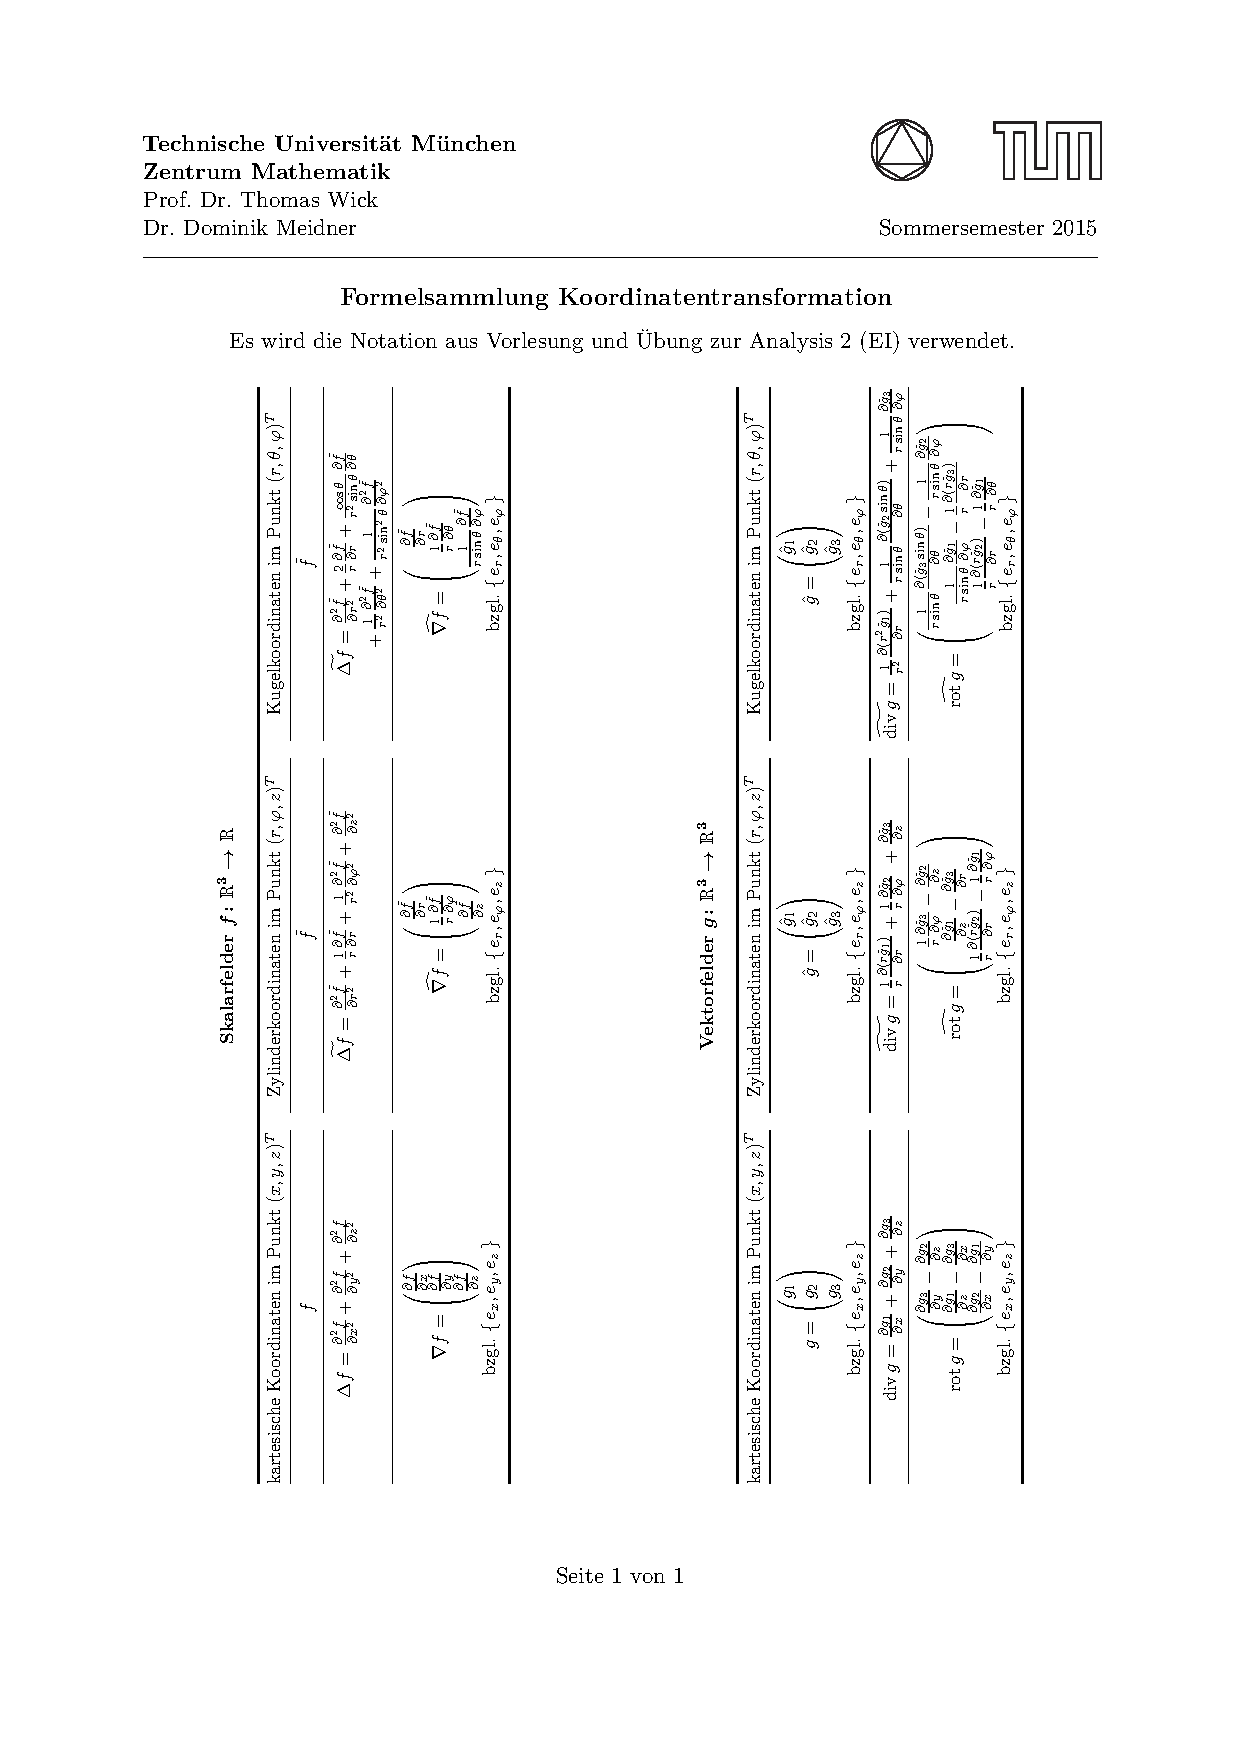
\includepdf[angle=-90]{./img/koordinaten.pdf}

\setlength\extrarowheight{5pt}
\section{Anhang: Krummlinige Koordinaten}
\begin{center}
    \begin{tabular}{|c|c|c|c|}
        \hline
                                  & \multicolumn{3}{c|}{\textbf{Skalarfelder $f:\mathbb{R}^3\rightarrow\mathbb{R}$}}                                                                                                                                                                                                                                                                                                                                                                                                                                                                                                                                                                             \\
        \hline
        \textbf{Koordinatentyp}   & karthesische Koordinaten im Punkt $(x,y,z)^T$                                                                 & Zylinderkoordinaten im Punkt $(r,\varphi,z)^T$                                                                                                                                                                      & Kugelkoordinaten um Punkt $(r,\varphi,\theta)^T$                                                                                                                                                                                                                                                                       \\
        \hline
                                  & $f$                                                                                                           & $\tilde{f}$                                                                                                                                                                                                         & $\tilde{f}$                                                                                                                                                                                                                                                                                                            \\
        \hline
        \textbf{Laplace-Operator} & $\Delta f=\frac{\partial^2f}{\partial x^2}+\frac{\partial^2f}{\partial y^2}+\frac{\partial^2f}{\partial z^2}$ & $\widetilde{\Delta f}=\frac{\partial^2\tilde{f}}{\partial r^2}+\frac{1}{r}\frac{\partial\tilde{f}}{\partial r}+\frac{1}{r^2}\frac{\partial^2\tilde{f}}{\partial\varphi^2}+\frac{\partial^2\tilde{f}}{\partial z^2}$ & $\widetilde{\Delta f}=\frac{\partial^2\tilde{f}}{\partial r^2}+\frac{2}{r}\frac{\partial\tilde{f}}{\partial r}+\frac{1}{r^2sin^2\theta}\frac{\partial^2\tilde{f}}{\partial\varphi^2}+\frac{cos\theta}{r^2sin\theta}\frac{\partial\tilde{f}}{\partial\theta}+\frac{1}{r^2}\frac{\partial^2\tilde{f}}{\partial\theta^2}$ \\
        \hline
        \textbf{Gradient}         & $\nabla f=\begin{pmatrix} \frac{\partial f}{\partial x} \\ \frac{\partial f}{\partial y} \\ \frac{\partial f}{\partial z} \end{pmatrix}$                                                                         & $\widehat{\nabla f}=\begin{pmatrix} \frac{\partial\tilde{f}}{\partial r} \\ \frac{1}{r}\frac{\partial\tilde{f}}{\partial\varphi} \\ \frac{\partial\tilde{f}}{\partial z} \end{pmatrix}$                                                                                                                                                                     & $\widehat{\nabla f}=\begin{pmatrix} \frac{\partial\tilde{f}}{\partial r} \\ \frac{1}{r\cdot sin\theta}\frac{\partial\tilde{f}}{\partial\varphi} \\ \frac{1}{r}\frac{\partial\tilde{f}}{\partial\theta} \end{pmatrix}$                                                                                                                                                                                                                                                                        \\
        \hline
        \textbf{Basis}            & $\{e_x,e_y,e_z\}$                                                                                             & $\{e_r,e_\varphi,e_z\}$                                                                                                                                                                                             & $\{e_r,e_\varphi,e_\theta\}$                                                                                                                                                                                                                                                                                           \\
        \hline
        %%        \end{tabular}
        %%        \begin{tabular}{|c|c|c|c|}
        %%            \hline
                                  & \multicolumn{3}{c|}{\textbf{Vektorfelder $g:\mathbb{R}^3\rightarrow\mathbb{R}^3$}}                                                                                                                                                                                                                                                                                                                                                                                                                                                                                                                                                                           \\
        \hline
        \textbf{Koordinatentyp}   & karthesische Koordinaten im Punkt $(x,y,z)^T$                                                                 & Zylinderkoordinaten im Punkt $(r,\varphi,z)^T$                                                                                                                                                                      & Kugelkoordinaten um Punkt $(r,\varphi,\theta)^T$                                                                                                                                                                                                                                                                       \\
        \hline
                                  & $g=\begin{pmatrix} g_1 \\ g_2 \\ g_3 \end{pmatrix}$                                                                                & $\hat{g}=\begin{pmatrix} \hat{g}_1 \\ \hat{g}_2 \\ \hat{g}_3 \end{pmatrix}$                                                                                                                                                                                & $\hat{g}=\begin{pmatrix} \hat{g}_1 \\ \hat{g}_2 \\ \hat{g}_3 \end{pmatrix}$                                                                                                                                                                                                                                                                                   \\
        \hline
        \textbf{Divergenz}        & $\text{div}g=\frac{\partial g_1}{\partial x}+\frac{\partial g_2}{\partial y}+\frac{\partial g_3}{\partial z}$ & $\widetilde{\text{div}g}=\frac{1}{r}\frac{\partial(r\hat{g}_1)}{\partial r}+\frac{1}{r}\frac{\partial\hat{g}_2}{\partial\varphi}+\frac{\partial\hat{g}_3}{\partial z}$                                              & $\widetilde{\text{div}g}=\frac{1}{r2}\frac{\partial(r^2\hat{g}_1)}{\partial r}+\frac{1}{r\cdot sin\theta}\frac{\partial\hat{g}_2}{\partial\varphi}+\frac{1}{r\cdot sin\theta}\frac{\partial(\hat{g}_3sin\theta)}{\partial\theta}$                                                                                      \\
        \hline
        \textbf{Rotation}         & $\text{rot}g=\begin{pmatrix} \frac{\partial g_3}{\partial y}-\frac{\partial g_2}{\partial z} \\ \frac{\partial g_1}{\partial z}-\frac{\partial g_3}{\partial x} \\ \frac{\partial g_2}{\partial x}-\frac{\partial g_1}{\partial y} \end{pmatrix}$                                                                      & $\widehat{\text{rot}g}=\begin{pmatrix} \frac{1}{r}\frac{\partial\hat{g}_3}{\partial\varphi}-\frac{\partial\hat{g}_2}{\partial z} \\ \frac{\partial\hat{g}_1}{\partial z}-\frac{\partial\hat{g}_3}{\partial r} \\ \frac{1}{r}\frac{\partial(r\hat{g}_2)}{\partial r}-\frac{1}{r}\frac{\partial\hat{g}_1}{\partial\varphi} \end{pmatrix}$                                                                                                                                                                  & $\widehat{\text{rot}g}=\begin{pmatrix} \frac{1}{r\cdot sin\theta}\frac{\partial(\hat{g}_2sin\theta)}{\partial\theta}-\frac{1}{r\cdot sin\theta}\frac{\partial\hat{g}_3}{\partial\varphi} \\ \frac{1}{r}\frac{\partial(r\hat{g}_3)}{\partial r}-\frac{1}{r}\frac{\partial\hat{g}_1}{\partial\theta} \\ \frac{1}{r\cdot sin\theta}\frac{\partial\hat{g}_1}{\partial\varphi}-\frac{1}{r}\frac{\partial(r\hat{g}_2)}{\partial r} \end{pmatrix}$                                                                                                                                                                                                                                                                     \\
        \hline
        \textbf{Basis}            & $\{e_x,e_y,e_z\}$                                                                                             & $\{e_r,e_\varphi,e_z\}$                                                                                                                                                                                             & $\{e_r,e_\varphi,e_\theta\}$                                                                                                                                                                                                                                                                                           \\
        \hline
    \end{tabular}
\end{center}
\textbf{Umrechnung zwischen den Koordinatensystemen:}
\begin{center}
    \begin{tabular}{|ccc|c|c|c|}
        \hline
        Zylinderkoordinaten     & $\Rightarrow$ & kartesische Koordinanten & $x=r\cdot cos\varphi$                & $y=r\cdot sin\varphi$                                                                            & $z=z$                                                \\
        \hline
        kartesische Koordinaten & $\Rightarrow$ & Zylinderkoordinaten      & $r=\sqrt{x^2+y^2}$                   & $\varphi=arccos\frac{x}{\sqrt{x^2+y^2}}=arctan\frac{y}{x}$                                       & $z=z$                                                \\
        \hline
        Kugelkoordinaten        & $\Rightarrow$ & kartesische Koordinaten  & $x=r\cdot sin\theta\cdot cos\varphi$ & $y=r\cdot sin\theta\cdot sin\varphi$                                                             & $z=r\cdot cos\theta$                                 \\
        \hline
        kartesische Koordinaten & $\Rightarrow$ & Kugelkoordinaten         & $r=\sqrt{x^2+y^2+z^2}$               & $cos\varphi=\frac{x}{\sqrt{x^2+y^2}};sin\varphi=\frac{y}{\sqrt{x^2+y^2}};tan\varphi=\frac{y}{x}$ & $cos\theta=\frac{z}{r}=\frac{z}{\sqrt{x^2+y^2+z^2}}$ \\
        \hline
        Kugelkoordinaten        & $\Rightarrow$ & Zylinderkoordinaten      & $r_z=r_k\cdot sin\theta$             & $\varphi_z=\varphi_k$                                                                            & $z_z=r_k\cdot\cos\theta$                             \\
        \hline
        Zylinderkoordinaten     & $\Rightarrow$ & Kugelkoordinaten         & $r_k=\sqrt{r_z^2+z_z^2}$             & $\varphi_k=\varphi_z$                                                                            & $\theta=arctan\frac{r_z}{z_z}$                       \\
        \hline
    \end{tabular} \\
    Quelle: http://www.calc3d.com/help/gcoord.html
\end{center}

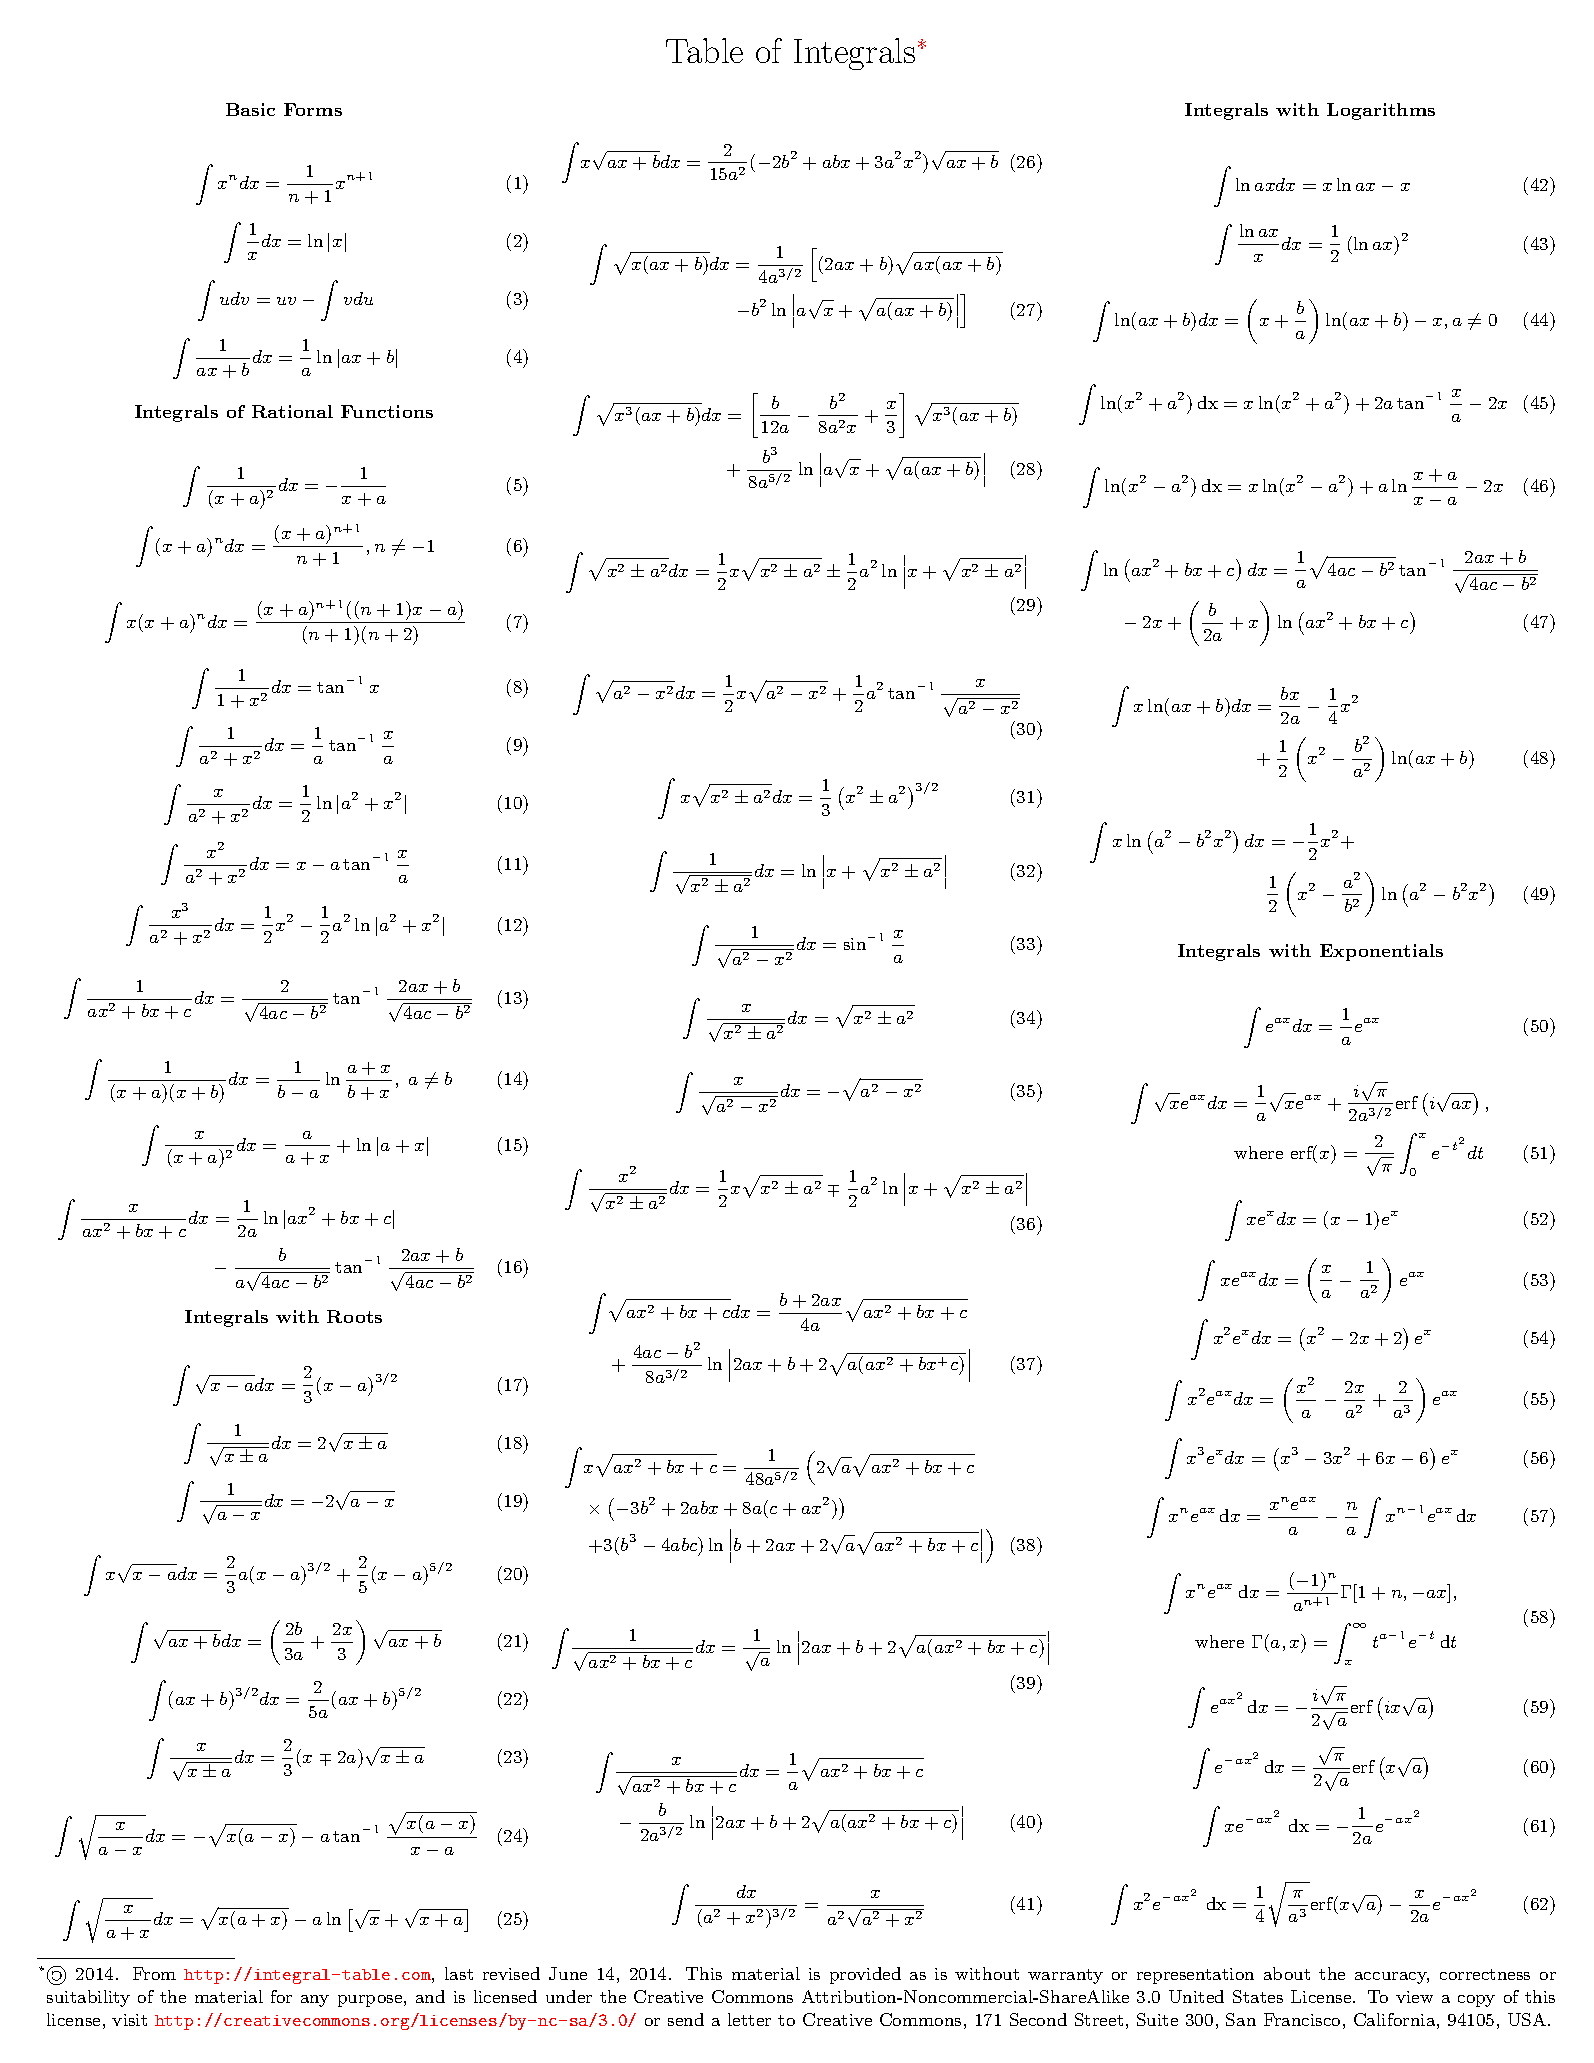
\includepdf[pages={1-2}, angle=-90]{./img/single-page-integral-table.pdf}
% Dokumentende
% ======================================================================
\end{document}
